%═══════════════════════════════════════════════════════════════════════════════
\chapter{Arquitecturas especializadas: inductive bias y simetría}
\label{ch:cap9}
%═══════════════════════════════════════════════════════════════════════════════

El MLP denso del Capítulo~\ref{ch:cap4} es un aproximador universal: puede representar
cualquier función continua con precisión arbitraria. Pero la universalidad tiene
un precio. El espacio de hipótesis es tan grande que el modelo necesita muchos
datos para identificar la función correcta entre todas las posibles. Cuando el
problema tiene estructura conocida —simetría bajo traslación, permutación,
rotación, o algún grupo de Lie más general— esa universalidad es un exceso que
se paga con mala generalización en el régimen de datos moderados.

El principio que organiza este capítulo es el \textbf{inductive bias estructural}:
codificar en la arquitectura las simetrías del problema restringe el espacio de
hipótesis al subconjunto de funciones compatibles con esas simetrías, reduciendo
drásticamente la complejidad efectiva del modelo y mejorando la generalización
sin sacrificar la capacidad de aproximar las funciones relevantes. Este principio
no es una heurística de ingeniería: es una consecuencia del Lema de Schur de la
teoría de representaciones de grupos, que determina completamente la estructura
permitida de las capas lineales para cualquier grupo de simetría dado.

Las cuatro arquitecturas del capítulo (CNNs, GNNs, transformers, redes
equivariantes de grupo) son casos particulares del mismo marco. Las conexiones
residuales y las Neural ODEs cierran el capítulo vinculando las redes profundas
con los sistemas dinámicos, preparando el terreno para los modelos de difusión
del Capítulo~\ref{ch:cap12}.

%───────────────────────────────────────────────────────────────────────────────
\section{Inductive bias: estructurar el espacio de hipótesis}
\label{sec:inductive_bias}
\dificultad{2}{1}
%───────────────────────────────────────────────────────────────────────────────

\subsection{El costo de la universalidad}
\label{subsec:costo_universalidad}

Sea $\mathcal{F}$ la clase de funciones que un MLP denso puede representar y
$\mathcal{F}_G \subset \mathcal{F}$ el subconjunto de funciones $G$-equivariantes.
El cociente $|\mathcal{F}|/|\mathcal{F}_G|$ mide cuánto se reduce el espacio de
búsqueda al imponer la simetría. Para el grupo de permutaciones $S_n$,
$|\mathcal{F}|/|\mathcal{F}_{S_n}| = n!$: trabajar con funciones sin
estructura permutacional es factorialmente más costoso que trabajar con funciones
simétricas.

\begin{proposicion}{Reducción de VC-dimensión bajo simetría}
\label{prop:vc_simetria}
Sea $G$ un grupo finito de orden $|G|$ que actúa sobre $\mathcal{X}$ y sea
$\mathcal{F}_G$ la clase de clasificadores $G$-invariantes restringidos de una
clase $\mathcal{F}$ con VC-dimensión $d$. Entonces
$\mathrm{VCdim}(\mathcal{F}_G) \leq d/|G|$.
\end{proposicion}

\begin{proof}
Si $\mathcal{F}_G$ fragmenta un conjunto $S = \{\bm{x}_1,\ldots,\bm{x}_m\}$,
entonces fragmenta también las $|G|$ órbitas de cada punto. Para cada etiquetado
de $S$, el clasificador $G$-invariante produce el mismo etiquetado en todos los
elementos de la órbita. El número de etiquetados distinguibles es a lo sumo
$2^{m/|G|}$, mientras que fragmentar $S$ requiere $2^m$ etiquetados. Por tanto
$m/|G| \leq d$, es decir $m \leq d|G|/|G| = d$. Más precisamente,
$\mathrm{VCdim}(\mathcal{F}_G) \leq \lfloor d/|G| \rfloor$. $\square$
\end{proof}

\subsection{Simetría, equivarianza e invarianza}
\label{subsec:equivarianza}

\begin{definicion}{Acción de grupo y equivarianza}
\label{def:equivarianza}
Sea $G$ un grupo que actúa sobre $\mathcal{X}$ mediante la representación
$\rho_{\mathrm{in}}: G \to \mathrm{Aut}(\mathcal{X})$ y sobre $\mathcal{Y}$
mediante $\rho_{\mathrm{out}}: G \to \mathrm{Aut}(\mathcal{Y})$.
Una función $f: \mathcal{X} \to \mathcal{Y}$ es:
\begin{itemize}
  \item \textbf{$G$-equivariante} si $f(\rho_{\mathrm{in}}(g)\bm{x})
        = \rho_{\mathrm{out}}(g)f(\bm{x})$ para todo $g \in G$,
        $\bm{x} \in \mathcal{X}$.
  \item \textbf{$G$-invariante} si $f(\rho_{\mathrm{in}}(g)\bm{x})
        = f(\bm{x})$ para todo $g \in G$ (caso $\rho_{\mathrm{out}} = \mathrm{id}$).
\end{itemize}
\end{definicion}

La equivarianza expresa que transformar la entrada y luego aplicar $f$ es lo
mismo que aplicar $f$ y luego transformar la salida: la función respeta la
acción del grupo. La invarianza es el caso donde la salida no se transforma.

\subsection{El Lema de Schur y la estructura de las capas equivariantes}
\label{subsec:schur}

\begin{teorema}{Lema de Schur}
\label{lema:schur}
Sea $G$ un grupo y $\rho_1: G \to \mathrm{GL}(V_1)$, $\rho_2: G \to
\mathrm{GL}(V_2)$ dos representaciones irreducibles de $G$ sobre un cuerpo
algebraicamente cerrado $\mathbb{F}$. Sea $\phi: V_1 \to V_2$ un mapa lineal
tal que $\phi\circ\rho_1(g) = \rho_2(g)\circ\phi$ para todo $g \in G$
(\textbf{mapa entretejedor}). Entonces:
\begin{enumerate}
  \item Si $\rho_1 \not\cong \rho_2$ (no isomorfas), entonces $\phi = 0$.
  \item Si $\rho_1 \cong \rho_2$ y $\mathbb{F} = \mathbb{C}$, entonces
        $\phi = \lambda\,\mathrm{id}$ para algún $\lambda \in \mathbb{C}$.
\end{enumerate}
\end{teorema}

El Lema de Schur tiene una consecuencia directa para el diseño de capas
equivariantes. Sea $\bm{W}: \mathbb{R}^{n_{\mathrm{in}}} \to
\mathbb{R}^{n_{\mathrm{out}}}$ una capa lineal equivariante respecto a
representaciones $\rho_{\mathrm{in}}$ y $\rho_{\mathrm{out}}$ de $G$.
La condición de equivarianza es $\bm{W}\rho_{\mathrm{in}}(g) =
\rho_{\mathrm{out}}(g)\bm{W}$ para todo $g \in G$.

Por el teorema de descomposición de Maschke, toda representación de un grupo
finito (o compacto) sobre $\mathbb{R}$ se descompone en suma directa de
irreducibles: $\rho_{\mathrm{in}} = \bigoplus_\alpha m_\alpha^{\mathrm{in}}
\rho_\alpha$ y $\rho_{\mathrm{out}} = \bigoplus_\beta m_\beta^{\mathrm{out}}
\rho_\beta$, donde $m_\alpha$ es la multiplicidad del irreducible $\rho_\alpha$.
En la base de bloques irreducibles, el Lema de Schur implica que $\bm{W}$ solo
puede conectar bloques irreducibles del mismo tipo y que, dentro de cada tipo,
actúa como un múltiplo escalar de la identidad. Los únicos parámetros libres
son los coeficientes de esos múltiplos escalares.

Esta es la \textbf{forma canónica de una capa equivariante}: las CNNs, GNNs y
redes equivariantes de $\mathrm{SO}(3)$ son todas consecuencias de esta forma
para grupos distintos.

%───────────────────────────────────────────────────────────────────────────────
\section{Redes convolucionales: equivarianza de traslación}
\label{sec:cnn}
\dificultad{2}{2}
%───────────────────────────────────────────────────────────────────────────────

\subsection{El grupo de traslaciones y la convolución}
\label{subsec:translacion}

Para datos sobre la cuadrícula $\mathbb{Z}^d$ (imágenes, series temporales,
volúmenes), el grupo natural de simetría es el grupo de traslaciones
$G = (\mathbb{Z}^d, +)$ con acción $(T_{\bm{v}}f)[\bm{x}] = f[\bm{x}-\bm{v}]$.

\begin{teorema}{La convolución como única capa lineal equivariante bajo traslación}
\label{thm:conv_equivar}
Una capa lineal $\Phi: L^2(\mathbb{Z}^d) \to L^2(\mathbb{Z}^d)$ es equivariante
bajo traslaciones (es decir, $\Phi \circ T_{\bm{v}} = T_{\bm{v}} \circ \Phi$
para todo $\bm{v} \in \mathbb{Z}^d$) si y solo si es una convolución discreta:
\[
  (\Phi f)[\bm{x}] = (f * k)[\bm{x}] = \sum_{\bm{v} \in \mathbb{Z}^d}
  k[\bm{v}]\,f[\bm{x}-\bm{v}],
\]
para algún núcleo $k: \mathbb{Z}^d \to \mathbb{R}$.
\end{teorema}

\begin{proof}
(\textbf{Suficiencia}) Si $\Phi = k*$, entonces
$(\Phi \circ T_{\bm{v}}f)[\bm{x}] = \sum_{\bm{u}} k[\bm{u}] f[\bm{x}-\bm{v}-\bm{u}]$
y $(T_{\bm{v}} \circ \Phi f)[\bm{x}] = \sum_{\bm{u}} k[\bm{u}] f[\bm{x}-\bm{v}-\bm{u}]$:
coinciden.

(\textbf{Necesidad}) Sea $\Phi$ equivariante. Definir $k[\bm{v}] = (\Phi\delta_{\bm{0}})[\bm{v}]$
donde $\delta_{\bm{0}}$ es la función impulso en el origen. Para cualquier $f$,
$f[\bm{x}] = \sum_{\bm{v}} f[\bm{v}]\,\delta_{\bm{0}}[\bm{x}-\bm{v}]$.
Por linealidad y equivarianza:
\[
  (\Phi f)[\bm{x}]
  = \sum_{\bm{v}} f[\bm{v}]\,(\Phi\delta_{\bm{0}})[\bm{x}-\bm{v}]
  = \sum_{\bm{v}} f[\bm{v}]\,k[\bm{x}-\bm{v}]
  = (f*\tilde{k})[\bm{x}],
\]
donde $\tilde{k}[\bm{v}] = k[-\bm{v}]$. Redefiniendo $k$ apropiadamente se
obtiene la convolución. $\square$
\end{proof}

La CNN no es una elección empírica motivada por la biología del córtex visual:
es la consecuencia algebraica necesaria de imponer equivarianza de traslación.

\begin{fisicaconexion}{Convolución en óptica física y procesado de señales}
El Teorema~\ref{thm:conv_equivar} tiene una manifestación directa en óptica: un
sistema óptico \textbf{lineal e isoplanático} (que responde igual a un objeto
sin importar su posición en el campo) produce en el plano imagen la convolución
del objeto con su \textbf{función de dispersión puntual} (PSF):
\[
  I_{\text{imagen}}(\bm{x})
  = \int \mathrm{PSF}(\bm{x}-\bm{x}')\,I_{\text{objeto}}(\bm{x}')\,d\bm{x}'.
\]
La isoplanatia es exactamente la equivarianza de traslación: el sistema óptico
trata igual a un punto en el centro que en el borde del campo. La
\textbf{función de transferencia óptica} (OTF) es la transformada de Fourier de
la PSF; un sistema de difracción limitada tiene OTF igual al disco de Airy,
mientras que las aberraciones modifican su fase (función de aberración de onda).
La deconvolución de imágenes astronómicas —recuperar la imagen verdadera a
partir de la imagen borrosa producida por la atmósfera— es el problema inverso
de esta convolución, análogo al filtro de Tikhonov del Capítulo~\ref{ch:cap2}.

En procesado de señales 1D, un filtro lineal invariante en el tiempo (LTI) está
completamente caracterizado por su respuesta al impulso $h(t)$, y la salida es
la convolución $y(t) = (x * h)(t)$. El \textbf{teorema de convolución de
Fourier}, $\mathcal{F}\{x*h\} = \mathcal{F}\{x\}\cdot\mathcal{F}\{h\}$,
convierte la convolución ($O(n^2)$) en multiplicación puntual en frecuencia,
implementable en $O(n\log n)$ vía FFT. Los núcleos aprendidos de una CNN son
filtros cuyas respuestas en frecuencia el modelo determina a partir de los datos:
un filtro de diferencias finitas $k = (1,-2,1)$ es un detector de curvatura
(laplaciano discreto); el gradiente de una CNN en las capas tempranas aprende
filtros de bordes análogos a los filtros de Sobel.
\end{fisicaconexion}

\subsection{La capa convolucional: parámetros y backpropagation}
\label{subsec:capa_conv}

Para $C_{\mathrm{in}}$ canales de entrada y $C_{\mathrm{out}}$ de salida, el
núcleo es $\bm{K} \in \mathbb{R}^{C_{\mathrm{out}} \times C_{\mathrm{in}}
\times h \times w}$:
\[
  Z_{c,\bm{x}} = \sum_{c'=1}^{C_{\mathrm{in}}}
  \sum_{\bm{v} \in \mathcal{N}} K_{c,c',\bm{v}}\,A_{c',\bm{x}-\bm{v}} + b_c,
\]
con $|\mathcal{N}| = h \cdot w$ posiciones del núcleo. El número de parámetros
es $C_{\mathrm{out}} C_{\mathrm{in}} h w$: independiente del tamaño espacial $n$.
Para una capa densa equivalente sería $C_{\mathrm{out}} C_{\mathrm{in}} n^2$.

El backward pass de la convolución es una convolución con núcleo transpuesto:
\[
  \frac{\partial\mathcal{L}}{\partial K_{c,c',\bm{v}}}
  = \sum_{\bm{x}} \delta_{c,\bm{x}}\,A_{c',\bm{x}-\bm{v}},
  \qquad
  \frac{\partial\mathcal{L}}{\partial A_{c',\bm{x}}}
  = \sum_c \sum_{\bm{v}} K_{c,c',\bm{v}}\,\delta_{c,\bm{x}+\bm{v}}.
\]
La primera es la correlación cruzada entre el error $\bm{\delta}$ y la activación
de entrada; la segunda es la convolución del error con el núcleo volteado.
Backpropagation en una CNN es una CNN aplicada en sentido inverso.

%───────────────────────────────────────────────────────────────────────────────
\section{Redes de grafos: equivarianza de permutación}
\label{sec:gnn}
\dificultad{2}{2}
%───────────────────────────────────────────────────────────────────────────────

\subsection{Datos con estructura de grafo y el grupo $S_n$}
\label{subsec:datos_grafo}

Sea un grafo $\mathcal{G} = (\mathcal{V}, \mathcal{E})$ con $n = |\mathcal{V}|$
nodos y características $\bm{X} \in \mathbb{R}^{n \times d}$,
$\bm{E} \in \mathbb{R}^{|\mathcal{E}| \times d_e}$. Una permutación
$\pi \in S_n$ actúa permutando las filas de $\bm{X}$ y las aristas de
$\bm{E}$ consistentemente. Una función sobre grafos que sea independiente
del etiquetado de los nodos debe ser $S_n$-invariante.

\subsection{DeepSets: el teorema de representación para conjuntos}
\label{subsec:deepsets}

\begin{teorema}{Representación de funciones invariantes bajo permutación}
\label{thm:deepsets}
Sea $f: \mathcal{X}^n \to \mathbb{R}$ una función continua invariante bajo
permutaciones del conjunto de entrada $\{\bm{x}_1,\ldots,\bm{x}_n\} \subset
\mathcal{X} \subset \mathbb{R}^d$ con $\mathcal{X}$ compacto. Entonces existen
funciones continuas $\phi: \mathcal{X} \to \mathbb{R}^M$ y
$\rho: \mathbb{R}^M \to \mathbb{R}$ tales que:
\[
  f(\bm{x}_1,\ldots,\bm{x}_n)
  = \rho\!\left(\sum_{i=1}^n \phi(\bm{x}_i)\right).
\]
\end{teorema}

\begin{proof}
(\textbf{Esquema}) Se construye explícitamente $\phi$ y $\rho$.
Para $\mathcal{X} \subset \mathbb{R}$ (caso escalar, la generalización a
$\mathbb{R}^d$ es análoga), elegir $M > n$ y definir la función de suma de
potencias $\phi(x) = (x, x^2, \ldots, x^M)$: el vector $\sum_i \phi(x_i) =
(\sum_i x_i, \sum_i x_i^2, \ldots, \sum_i x_i^M)$ son los polinomios de
Newton del conjunto $\{x_1,\ldots,x_n\}$. Por las identidades de Newton entre
polinomios de Newton y polinomios simétricos elementales, y por el teorema
fundamental de los polinomios simétricos, los polinomios de Newton determinan
únicamente el multiconjunto $\{x_1,\ldots,x_n\}$ cuando $M \geq n$. Luego
$\rho$ puede reconstruir $f$ a partir de $\sum_i\phi(x_i)$.

Para $\mathcal{X} \subset \mathbb{R}^d$, Zaheer et al.\ (2017) muestran que
una función genérica $\phi: \mathbb{R}^d \to \mathbb{R}^M$ con $M$ suficientemente
grande es inyectiva sobre multiconjuntos finitos, lo que permite reconstruir
$f$ mediante $\rho$. $\square$
\end{proof}

La arquitectura \textbf{DeepSets} implementa exactamente este teorema:
$\phi$ y $\rho$ son MLPs. La suma $\sum_i \phi(\bm{x}_i)$ es el único
agregador lineal equivariante (invariante a permutaciones): cualquier otro
agregador simétrico (media, máximo, mínimo) puede obtenerse combinando sumas.

\subsection{Message passing: la GNN general}
\label{subsec:message_passing}

\begin{definicion}{Red neuronal de paso de mensajes (MPNN)}
\label{def:mpnn}
Una \textbf{MPNN} con $T$ iteraciones tiene la forma:
\begin{align}
  \bm{m}_{ij}^{(t)}
  &= \phi_m\!\left(\bm{h}_i^{(t)},\, \bm{h}_j^{(t)},\, \bm{e}_{ij}\right),
  \tag{mensaje} \label{eq:mensaje}\\
  \bm{h}_i^{(t+1)}
  &= \phi_h\!\left(\bm{h}_i^{(t)},\,
    \bigoplus_{j \in \mathcal{N}(i)} \bm{m}_{ij}^{(t)}\right),
  \tag{actualización} \label{eq:actualizacion}\\
  \hat{y}
  &= \phi_g\!\left(\bigoplus_{i \in \mathcal{V}} \bm{h}_i^{(T)}\right),
  \tag{readout} \label{eq:readout}
\end{align}
donde $\bm{h}_i^{(0)} = \bm{x}_i$, $\bigoplus$ es un agregador invariante
bajo permutación (suma, media, max), y $\phi_m$, $\phi_h$, $\phi_g$ son MLPs.
\end{definicion}

La MPNN es equivariante bajo permutación de nodos por construcción: los mensajes
y las actualizaciones son funciones de pares (nodo, vecinos), y el agregador
$\bigoplus$ elimina el orden de los vecinos.

\subsection{Expresividad de las GNNs y el test de Weisfeiler-Leman}
\label{subsec:wl}

\subsubsection*{El algoritmo de Weisfeiler-Leman (WL-1)}

El test de isomorfismo de grafos de Weisfeiler-Leman de primer orden (WL-1)
asigna colores a los nodos iterativamente:
\begin{enumerate}
  \item Inicializar: $c_i^{(0)} = \mathrm{hash}(\bm{x}_i)$ para cada nodo.
  \item Iterar: $c_i^{(t+1)} = \mathrm{hash}\!\left(c_i^{(t)},
        \{\!\{ c_j^{(t)} : j \in \mathcal{N}(i) \}\!\}\right)$,
        donde $\{\!\{\cdot\}\!\}$ denota un multiconjunto.
  \item Detener cuando no hayan cambios en los colores.
\end{enumerate}
Dos grafos son declarados no isomorfos si y solo si producen histogramas de
colores distintos en alguna iteración. WL-1 no siempre es correcto: hay grafos
no isomorfos que produce el mismo histograma.

\subsubsection*{Equivalencia entre MPNNs y WL-1}

\begin{teorema}{Expresividad de las MPNNs (Xu et al., 2019)}
\label{thm:gnn_wl}
\begin{enumerate}
  \item Toda MPNN que es tan o más expresiva que WL-1 no puede distinguir
        grafos que WL-1 tampoco distingue.
  \item Existe una MPNN (la GIN, \textit{Graph Isomorphism Network}) que
        es exactamente tan expresiva como WL-1.
\end{enumerate}
\end{teorema}

\begin{proof}
\textbf{Parte 1} (cota superior de expresividad).
Sea $\mathcal{G}_1$ y $\mathcal{G}_2$ dos grafos tales que WL-1 no los distingue.
Se demostrará por inducción que ninguna MPNN puede asignar embeddings distintos
a nodos con el mismo color WL-1.

\textit{Caso base $t=0$:} WL-1 inicializa con $c_i^{(0)} = \mathrm{hash}(\bm{x}_i)$.
Si dos nodos $u \in \mathcal{G}_1$ y $v \in \mathcal{G}_2$ tienen el mismo
color inicial, entonces $\bm{x}_u = \bm{x}_v$, y la MPNN inicializa con
$\bm{h}_u^{(0)} = \phi_h(\bm{x}_u) = \phi_h(\bm{x}_v) = \bm{h}_v^{(0)}$.

\textit{Paso inductivo:} supóngase que en la iteración $t$, todos los nodos
con el mismo color WL-1 tienen el mismo embedding. La actualización de WL-1 es:
$c_i^{(t+1)} = \mathrm{hash}(c_i^{(t)}, \{\!\{c_j^{(t)}\}\!\}_{j\in\mathcal{N}(i)})$.
La actualización de la MPNN es:
$\bm{h}_i^{(t+1)} = \phi_h(\bm{h}_i^{(t)}, \bigoplus_{j\in\mathcal{N}(i)}
\phi_m(\bm{h}_i^{(t)},\bm{h}_j^{(t)}))$.

Si $c_u^{(t)} = c_v^{(t)}$ y $\{\!\{c_j^{(t)}: j\in\mathcal{N}(u)\}\!\} =
\{\!\{c_k^{(t)}: k\in\mathcal{N}(v)\}\!\}$ (misma condición que WL-1), entonces
por hipótesis inductiva $\bm{h}_j^{(t)} = \bm{h}_k^{(t)}$ para los vecinos
correspondientes, y la suma $\bigoplus_j \phi_m(\bm{h}_u^{(t)},\bm{h}_j^{(t)}) =
\bigoplus_k \phi_m(\bm{h}_v^{(t)},\bm{h}_k^{(t)})$. Luego
$\bm{h}_u^{(t+1)} = \bm{h}_v^{(t+1)}$.

Si WL-1 no puede distinguir $\mathcal{G}_1$ de $\mathcal{G}_2$, entonces
para cada nodo $u \in \mathcal{G}_1$ existe $v \in \mathcal{G}_2$ con el
mismo color en cada iteración, luego con el mismo embedding. El histograma
de embeddings de la MPNN tampoco distingue los grafos.

\textbf{Parte 2} (la GIN alcanza WL-1).
La GIN usa el agregador suma (el más poderoso entre los lineales, pues preserva
la multiplicidad) y la actualización:
\[
  \bm{h}_i^{(t+1)} = \phi_h\!\left((1+\epsilon)\bm{h}_i^{(t)}
  + \sum_{j\in\mathcal{N}(i)}\bm{h}_j^{(t)}\right),
\]
con $\phi_h$ una MLP suficientemente expresiva (capaz de inyectar multiconjuntos
en distintos vectores). Se demuestra que si $\phi_h$ es inyectiva sobre el espacio
de pares $(\bm{h}, \{\!\{\bm{h}_j\}\!\})$, la GIN puede distinguir todos los
grafos que WL-1 distingue.

La clave es que la suma $\sum_j \bm{h}_j$ (a diferencia de la media
$\frac{1}{|\mathcal{N}|}\sum_j \bm{h}_j$ o el max) preserva la información de
multiplicidad: $\{1,1,2\}$ y $\{1,2\}$ tienen la misma media y el mismo máximo,
pero sumas distintas. El parámetro $\epsilon$ rompe la posible confusión entre
el embedding del nodo propio y los de los vecinos. $\square$
\end{proof}

\subsubsection*{Grafos que WL-1 no puede distinguir y más allá}

WL-1 falla en distinguir grafos regulares del mismo grado y tamaño (por ejemplo,
el grafo ciclo $C_6$ y la unión de dos triángulos $K_3 \sqcup K_3$, ambos
3-regulares en 6 nodos). Para ir más allá de WL-1 existen dos estrategias:
\begin{itemize}
  \item \textbf{Características estructurales}: añadir a los nodos información
        sobre la estructura local (centralidad, conteo de ciclos,
        distancias). Esto rompe la simetría y puede aumentar la expresividad,
        pero tiene costo computacional adicional.
  \item \textbf{WL de orden superior}: el test $k$-WL considera $k$-tuplas de
        nodos en lugar de nodos individuales, con expresividad creciente en $k$.
        Las GNNs que implementan 3-WL pueden distinguir cualquier par de grafos
        no isomorfos que 3-WL distingue, pero la complejidad es $O(n^k)$.
\end{itemize}

%───────────────────────────────────────────────────────────────────────────────
\section{Mecanismo de atención y transformers}
\label{sec:attention}
\dificultad{2}{2}
%───────────────────────────────────────────────────────────────────────────────

\subsection{Atención escalada como producto interno}
\label{subsec:atencion}

\begin{definicion}{Atención escalada por producto interno}
\label{def:atencion}
Dada una secuencia de entrada $\bm{X} \in \mathbb{R}^{n\times d}$ y proyecciones
$\bm{W}_Q, \bm{W}_K \in \mathbb{R}^{d \times d_k}$, $\bm{W}_V \in \mathbb{R}^{d\times d_v}$:
\[
  \bm{Q} = \bm{X}\bm{W}_Q, \quad
  \bm{K} = \bm{X}\bm{W}_K, \quad
  \bm{V} = \bm{X}\bm{W}_V,
\]
\[
  \mathrm{Attn}(\bm{Q},\bm{K},\bm{V})
  = \mathrm{softmax}\!\left(\frac{\bm{Q}\bm{K}^\top}{\sqrt{d_k}}\right)\bm{V}
  \in \mathbb{R}^{n\times d_v}.
\]
\end{definicion}

El factor de escala $1/\sqrt{d_k}$ es necesario para estabilizar los gradientes.
Sin él, para $d_k$ grande, el producto $\bm{Q}\bm{K}^\top$ tiene entradas del
orden $\sqrt{d_k}$ (en media, si $\bm{q}_i$ y $\bm{k}_j$ tienen componentes
i.i.d.\ con media 0 y varianza 1, entonces $\bm{q}_i^\top\bm{k}_j \sim
\mathcal{N}(0,d_k)$). El softmax de argumentos de varianza $d_k$ produce
distribuciones casi degeneradas (una entrada cerca de 1, el resto cerca de 0),
con gradientes que se desvanecen. El factor $1/\sqrt{d_k}$ normaliza la
varianza a 1 antes del softmax.

\subsection{Atención multi-cabeza y el bloque transformer}
\label{subsec:transformer}

\begin{definicion}{Atención multi-cabeza y bloque transformer}
\label{def:transformer}
Con $H$ cabezas de atención con dimensiones $d_k = d_v = d/H$:
\[
  \mathrm{MHA}(\bm{X})
  = \mathrm{Concat}(\mathrm{head}_1,\ldots,\mathrm{head}_H)\bm{W}_O,
\]
\[
  \mathrm{head}_h = \mathrm{Attn}(\bm{X}\bm{W}_{Q,h},\bm{X}\bm{W}_{K,h},
  \bm{X}\bm{W}_{V,h}).
\]
El \textbf{bloque transformer} aplica MHA y una red de avance con conexiones
residuales y normalización de capa:
\begin{align*}
  \bm{X}' &= \mathrm{LN}(\bm{X} + \mathrm{MHA}(\bm{X})), \\
  \bm{X}'' &= \mathrm{LN}(\bm{X}' + \mathrm{FFN}(\bm{X}')),
\end{align*}
donde $\mathrm{FFN}(\bm{x}) = \bm{W}_2\,\mathrm{ReLU}(\bm{W}_1\bm{x}+\bm{b}_1)
+ \bm{b}_2$ se aplica independientemente a cada posición.
\end{definicion}

La atención sin codificación posicional es globalmente equivariante bajo
permutación de posiciones (como la GNN con agregación por suma). La
\textbf{codificación posicional} añade a cada posición $i$ un vector
$\bm{p}_i$ (sinusoidal o aprendido) que rompe esa simetría para secuencias
donde el orden importa. Sin codificación posicional, el transformer es
una GNN completamente conectada.

La complejidad de la atención es $O(n^2 d)$ en tiempo y $O(n^2)$ en memoria:
cuadrática en $n$. Para $n$ grande, se usan aproximaciones de bajo rango
(atención linealizada) o atención local por ventanas deslizantes.

En la formulación original de Vaswani et al.\ (2017),
la normalización se aplica \emph{después} de la conexión residual
(\textit{post-norm}):
$\bm{X}' = \mathrm{LN}(\bm{X} + \mathrm{MHA}(\bm{X}))$.
En la práctica moderna, la convención dominante es \textit{pre-norm}:
$\bm{X}' = \bm{X} + \mathrm{MHA}(\mathrm{LN}(\bm{X}))$.
La diferencia no es cosmética: la pre-norm estabiliza el flujo del
gradiente porque la señal de identidad de la conexión residual llega
a las capas anteriores sin pasar por la normalización.
La Sección~\ref{subsec:transformer_pde} muestra que esta distinción
tiene una interpretación precisa como condición de estabilidad
numérica de la EDP subyacente.


%────────────────────────────────────────────────────────────────
\subsection{El transformer como sistema dinámico continuo:
            una perspectiva de EDP}
\label{subsec:transformer_pde}
%────────────────────────────────────────────────────────────────

La descripción estándar del transformer es discreta y combinatoria:
$L$ bloques que se aplican en secuencia sobre una secuencia de $n$
tokens~\cite{vaswani2017attention}. Esta descripción es operacionalmente
completa pero oscurece por qué ciertos componentes —las conexiones
residuales, la normalización de capa— son necesarios en lugar de
convenientes. Una perspectiva de sistemas dinámicos disipa esa
oscuridad y produce intuición directamente transferible desde la
física computacional~\cite{transformer_pde_2024}.

%────────────────────────────────────────────────────────────────
\subsubsection*{Convención notacional}
%────────────────────────────────────────────────────────────────

Esta sección y la siguiente involucran cuatro variables de evolución
físicamente distintas. Para evitar ambigüedad con las variables
estocásticas de los Capítulos~\ref{ch:cap10}--\ref{ch:cap12}, se
adopta la siguiente convención, que se mantiene en el resto del
capítulo:

\begin{table}[h]
\centering
\caption{Variables de evolución del Capítulo~\ref{ch:cap9}.
         Cada variable tiene un rol físico distinto
         y no debe confundirse con las demás.}
\label{tab:notacion_evolucion}
\small
\begin{tabular}{llll}
\toprule
\textbf{Símbolo} & \textbf{Tipo} & \textbf{Rango} &
\textbf{Rol físico} \\
\midrule
$\ell \in \mathbb{Z}$ & Discreto & $\{0,\ldots,L\}$ &
  Índice de capa; profundidad discreta de la red \\
$\ell \in \mathbb{R}$ & Continuo & $[0,L]$ &
  Límite continuo del índice de capa (Neural ODE) \\
$t$ & Continuo & $[0,T]$ &
  Tiempo de difusión; nivel de ruido del proceso forward \\
$s$ & Continuo & $[0,t]$ &
  Variable de integración; tiempo del proceso reverso \\
\bottomrule
\end{tabular}
\end{table}

El símbolo $\ell$ se usa en ambos registros —discreto y continuo—
según el contexto: como superíndice $\bm{u}^{(\ell)}$ denota el
estado en la capa $\ell$-ésima; como argumento de una derivada
parcial $\partial/\partial\ell$ denota la profundidad continua.
Esta dualidad es análoga al uso de $t$ en los capítulos
estocásticos, donde $t$ designa simultáneamente el tiempo discreto
de los esquemas numéricos y el tiempo continuo del movimiento
browniano. El tiempo de difusión se reserva exclusivamente para
$t$ (Capítulos~\ref{ch:cap10}--\ref{ch:cap12}); nunca aparece como
argumento de las ecuaciones de esta sección.

%────────────────────────────────────────────────────────────────
\subsubsection*{El campo de información y sus dos dimensiones}
%────────────────────────────────────────────────────────────────

Sea $\bm{u}_i^{(\ell)} \in \mathbb{R}^d$ la representación del
token $i$ en la capa $\ell$. Se define el \textbf{campo de
información}:
\begin{equation}
  \bm{u}: \{1,\ldots,n\} \times \{0,\ldots,L\} \to \mathbb{R}^d,
  \qquad (i, \ell) \mapsto \bm{u}_i^{(\ell)}.
  \label{eq:campo_info}
\end{equation}
Este campo tiene dos dimensiones independientes: la
\textbf{dimensión espacial} $i$ (posición en la secuencia: tokens,
celdas de calorímetro, nodos de un grafo) y la \textbf{dimensión
de profundidad} $\ell$ (índice de capa, que juega el rol del tiempo
de evolución dentro de la red). El transformer evoluciona $\bm{u}$
desde el estado inicial $\bm{u}^{(0)}$ (embedding de la entrada)
hasta el estado final $\bm{u}^{(L)}$ (representación para la
predicción).

En el \textbf{límite continuo} $\ell \in [0,L]$, la evolución capa
a capa se aproxima por una EDP con variable independiente $\ell$.
La conexión residual
$\bm{u}^{(\ell+1)} = \bm{u}^{(\ell)} + F(\bm{u}^{(\ell)})$ es
exactamente el método de Euler con paso unitario para la ODE
$\partial_\ell\bm{u} = F(\bm{u})$, la misma correspondencia
establecida en la Sección~\ref{subsec:residual} para las
ResNets~\cite{chen2018neural}. La diferencia es que aquí $F$ depende
de \emph{todas} las posiciones $i$ simultáneamente, convirtiendo la
ODE en una EDP.

%────────────────────────────────────────────────────────────────
\subsubsection*{La ecuación maestra del transformer}
%────────────────────────────────────────────────────────────────

La evolución continua del campo de información está gobernada por
la \textbf{ecuación maestra}~\cite{transformer_pde_2024}:
\begin{equation}
  \frac{\partial \bm{u}(x,\ell)}{\partial \ell}
  = \underbrace{\mathcal{A}[\bm{u}](x,\ell)}_{\text{interacción no local}}
  + \underbrace{\mathcal{R}[\bm{u}](x,\ell)}_{\text{reacción local}}
  + \underbrace{\mathcal{D}[\bm{u}](x,\ell)}_{\text{difusión emergente}}
  + \underbrace{\mathcal{S}[\bm{u}](x,\ell)}_{\text{estabilización}},
  \label{eq:master_pde}
\end{equation}
donde $x$ es la coordenada espacial continua (posición del token) y
$\ell \in [0,L]$ es la profundidad continua. Esta ecuación gobierna
la evolución interna de la red durante una sola evaluación del
modelo. No debe confundirse con la ecuación de Fokker-Planck del
Capítulo~\ref{ch:cap11}, que gobierna la evolución de la densidad
de probabilidad $p_t(\bm{x})$ a lo largo del tiempo de difusión
$t$: son sistemas completamente distintos con variables de evolución
distintas ($\ell$ aquí, $t$ allá).

Los cuatro operadores tienen la misma jerarquía matemática y se
derivan a continuación con sus expresiones analíticas.

\medskip
\noindent\textbf{Operador de atención $\mathcal{A}$: interacción
no local.}
\begin{equation}
  \mathcal{A}[\bm{u}](x,\ell)
  = \int_\Omega K_{\mathrm{att}}\!\left(\bm{u}(x,\ell),\,
    \bm{u}(y,\ell)\right)
    \bm{W}_V\bm{u}(y,\ell)\,dy
  - \bm{u}(x,\ell),
  \label{eq:op_atencion}
\end{equation}
donde el núcleo de atención está determinado dinámicamente:
\[
  K_{\mathrm{att}}(\bm{u}(x),\bm{u}(y))
  = \frac{\exp\!\left(\bm{u}(x)^\top\bm{W}_Q^\top
    \bm{W}_K\,\bm{u}(y)/\sqrt{d_k}\right)}
  {\displaystyle\int_\Omega
    \exp\!\left(\bm{u}(x)^\top\bm{W}_Q^\top
    \bm{W}_K\,\bm{u}(z)/\sqrt{d_k}\right)dz}.
\]
El término $-\bm{u}(x,\ell)$ proviene de la conexión residual:
$\mathcal{A}$ es la corrección que la atención introduce sobre el
estado, no el estado mismo. La suma discreta $\sum_j \alpha_{ij}
\bm{V}(j)$ es la versión discreta de esta integral con pesos
$\alpha_{ij} = K_{\mathrm{att}}(\bm{u}_i, \bm{u}_j)$.

\begin{fisicaconexion}{Atención como operador integral de Fredholm}
La ecuación~\eqref{eq:op_atencion} tiene la forma exacta de un
\textbf{operador integral de Fredholm de segunda especie}:
$(\mathcal{K}f)(x) = \int K(x,y)f(y)\,dy - f(x)$,
con núcleo que depende no linealmente del estado. En física, esta
estructura aparece en la ecuación de transporte de Boltzmann
linealizada: el término de colisión
$\int \sigma(v,v')[f(v') - f(v)]\,dv'$ tiene la misma forma
—interacción no local con relajación hacia la media—,
con la diferencia de que el núcleo de Boltzmann está fijado por
la sección eficaz de colisión, mientras que el núcleo de atención
se aprende de los datos~\cite{villani2002review}.
\end{fisicaconexion}

\medskip
\noindent\textbf{Operador de reacción $\mathcal{R}$: transformación
local.}
\begin{equation}
  \mathcal{R}[\bm{u}](x,\ell)
  = \mathrm{FFN}(\bm{u}(x,\ell)) - \bm{u}(x,\ell),
  \qquad
  \mathrm{FFN}(\bm{z}) = \bm{W}_2\,\sigma(\bm{W}_1\bm{z}
  + \bm{b}_1) + \bm{b}_2.
  \label{eq:op_reaccion}
\end{equation}
El FFN actúa \emph{independientemente} en cada posición $x$: no
hay intercambio de información entre posiciones distintas. Es un
operador \textbf{local} en la dimensión espacial, análogo al término
de reacción $f(u)$ en una ecuación de reacción-difusión. La conexión
residual aparece explícitamente: $\mathcal{R}$ es la desviación del
FFN respecto a la identidad.

\medskip
\noindent\textbf{Operador de difusión $\mathcal{D}$: efecto emergente
de la codificación posicional.}

A diferencia de $\mathcal{A}$, $\mathcal{R}$ y $\mathcal{S}$, el
operador $\mathcal{D}$ no tiene un componente arquitectónico
exclusivo: \emph{emerge} de la interacción entre la codificación
posicional y el FFN. Su derivación sigue el mismo argumento que
justifica la ley de Fick como descripción macroscópica del
transporte microscópico~\cite{fick1855ueber, einstein1905bewegung}.

El FFN opera sobre la suma $\bm{u}_i + \bm{P}_i$, donde $\bm{P}_i
= \bm{P}(i)$ es la codificación posicional del token $i$.
Expandiendo en serie de Taylor alrededor de $\bm{u}_i$:
\begin{equation}
  \mathrm{FFN}(\bm{u}_i + \bm{P}_i)
  = \mathrm{FFN}(\bm{u}_i)
  + J_{\mathrm{FFN}}(\bm{u}_i)\,\bm{P}_i
  + \mathcal{O}(\|\bm{P}_i\|^2),
  \label{eq:taylor_ffn}
\end{equation}
donde $J_{\mathrm{FFN}}(\bm{u}_i) \in \mathbb{R}^{d\times d}$ es
la jacobiana del FFN evaluada en $\bm{u}_i$. El término de primer
orden en $\bm{P}_i$ contribuye a la variación espacial del campo
a través de las diferencias finitas entre posiciones adyacentes:
\begin{equation}
  J_{\mathrm{FFN}}(\bm{u}_i)\,
  \underbrace{(\bm{P}_{i+1} - 2\bm{P}_i + \bm{P}_{i-1})}_{\displaystyle
    \Delta^2_i\bm{P}\ \text{(laplaciano discreto)}}.
  \label{eq:laplaciano_discreto}
\end{equation}
Para codificaciones sinusoidales $P_k(i) = \sin(\omega_k i)$,
los modos son autofunciones del laplaciano continuo:
\begin{equation}
  \frac{d^2}{dx^2}\sin(\omega_k x) = -\omega_k^2\sin(\omega_k x),
  \label{eq:autofuncion_sin}
\end{equation}
por lo que en el límite continuo $\Delta^2_i\bm{P} \to
\partial_{xx}\bm{P}(x) = -\bm{\Omega}^2\bm{P}(x)$, con
$\bm{\Omega} = \mathrm{diag}(\omega_1,\ldots,\omega_d)$.
Sustituyendo en~\eqref{eq:laplaciano_discreto} y colectando los
términos de segundo orden en la ecuación de evolución:
\begin{equation}
  \boxed{
  \mathcal{D}[\bm{u}](x,\ell)
  = \nabla_x \cdot \!\left(D_{\mathrm{eff}}(\bm{u},x)\,
    \nabla_x\bm{u}\right),
  \quad
  D_{\mathrm{eff}}(\bm{u},x)
  \propto |\nabla_x\bm{P}(x)|^2\cdot
  \mathrm{Tr}(J_{\mathrm{FFN}}(\bm{u})).
  }
  \label{eq:op_difusion}
\end{equation}
El coeficiente $D_{\mathrm{eff}}$ depende del estado a través de
la traza de la jacobiana del FFN y de la posición a través del
gradiente de la codificación posicional: es una \textbf{difusión
no lineal y no homogénea}, con la misma estructura de la
ecuación de difusión porosa~\cite{vazquez2007porous} o el filtro
de Perona-Malik~\cite{perona1990scale}.

\begin{fisicaconexion}{$\mathcal{D}$ y la ley de Fick:
mismo estatus epistemológico}
La ley de Fick $\bm{J} = -D\nabla c$~\cite{fick1855ueber} no se
deriva de primeros principios: es la descripción constitutiva de
primer orden del transporte cuando el libre camino medio es
pequeño, cuya justificación estadística viene de que la caminata
aleatoria en el límite difusivo produce $\partial_t p =
D\nabla^2 p$~\cite{einstein1905bewegung}. El operador $\mathcal{D}$
tiene el \textbf{mismo estatus epistemológico}: es la descripción
macroscópica correcta del transporte emergente entre tokens
adyacentes, obtenida como límite continuo de la dinámica discreta
del FFN. Que $D_{\mathrm{eff}}$ sea no lineal y aprendido no lo
hace menos riguroso —es el análogo de $D(c)$ en medios
heterogéneos~\cite{bear1972dynamics}.
\end{fisicaconexion}

\begin{observacion}{Alcance: codificaciones sinusoidales
vs.\ patch embeddings}
\label{obs:difusion_alcance}
La derivación de~\eqref{eq:op_difusion} es exacta en el límite
continuo para codificaciones sinusoidales: la autopropiedad
bajo el laplaciano~\eqref{eq:autofuncion_sin} convierte el
término de segundo orden en un operador difusivo con coeficiente
analítico.

El \textbf{DiT}~\cite{peebles2023dit} del Capítulo~\ref{ch:cap12}
usa patch embeddings aprendidos, para los que la condición de
autofunción no se satisface y la expresión~\eqref{eq:op_difusion}
pierde su forma cerrada. El efecto difusivo persiste
—la expansión~\eqref{eq:taylor_ffn} sigue siendo válida— pero
$D_{\mathrm{eff}}$ depende de la geometría aprendida de los
embeddings y no es accesible analíticamente. En ese régimen,
$\mathcal{D}$ actúa como una \emph{inductive bias} difusiva
implícita cuya intensidad el modelo regula durante el
entrenamiento, y su función es absorbida parcialmente por
$\mathcal{A}$, que sobre patches espacialmente organizados
desarrolla patrones de atención local entre patches vecinos.
Los mapas de atención de las primeras capas de un DiT entrenado
deberían mostrar ese patrón: atención concentrada en vecindades
espaciales como evidencia empírica del mecanismo difusivo.
\end{observacion}

\medskip
\noindent\textbf{Operador de estabilización $\mathcal{S}$:
LayerNorm como control disipativo.}
\begin{equation}
  \mathcal{S}[\bm{u}](x,\ell)
  \approx -\gamma(x,\ell)\,
  \frac{\bm{u}(x,\ell) - \bm{\mu}_{\bm{u}}(\ell)}
  {\sqrt{\sigma^2_{\bm{u}}(\ell) + \epsilon}},
  \label{eq:op_estab}
\end{equation}
donde $\bm{\mu}_{\bm{u}}(\ell) = \int_\Omega \bm{u}(y,\ell)\,dy$
y $\sigma^2_{\bm{u}}(\ell) = \int_\Omega
\|\bm{u}(y,\ell)-\bm{\mu}_{\bm{u}}(\ell)\|^2\,dy$ son la media y
la varianza espaciales del campo en la profundidad $\ell$, y
$\gamma(x,\ell)$ es la magnitud de la corrección. El operador
$\mathcal{S}$ penaliza las desviaciones del campo respecto a su
media espacial: es un \textbf{amortiguamiento disipativo} que
suprime los modos de alta amplitud y previene el crecimiento
ilimitado de las activaciones.

\begin{table}[h]
\centering
\caption{Correspondencia entre arquitectura del transformer y
         operadores de la EDP maestra~\eqref{eq:master_pde}.
         La variable de evolución $\ell$ es la profundidad de
         la red (discreta o continua según el contexto);
         el tiempo de difusión $t$ de los capítulos estocásticos
         no interviene en esta ecuación.}
\label{tab:transformer_pde}
\small
\begin{tabular}{llll}
\toprule
\textbf{Componente} & \textbf{Operador} &
\textbf{Ecuación} & \textbf{Naturaleza} \\
\midrule
Auto-atención (MHA)
  & $\mathcal{A}[\bm{u}]$
  & \eqref{eq:op_atencion}
  & Integral de Fredholm, adaptativa \\
Red de avance (FFN)
  & $\mathcal{R}[\bm{u}]$
  & \eqref{eq:op_reaccion}
  & Reacción puntual, no lineal \\
Cod.\ posicional $+$ FFN
  & $\mathcal{D}[\bm{u}]$
  & \eqref{eq:op_difusion}
  & Difusión no lineal, emergente \\
LayerNorm (pre-norm)
  & $\mathcal{S}[\bm{u}]$
  & \eqref{eq:op_estab}
  & Amortiguamiento disipativo \\
Conexión residual
  & $+\bm{u}(x,\ell)$
  & —
  & Integrador de Euler, identidad \\
\midrule
Profundidad $\ell \in [0,L]$
  & Variable de evolución
  & — & — \\
Posición token $i \to x$
  & Coordenada espacial
  & — & — \\
\bottomrule
\end{tabular}
\end{table}

%────────────────────────────────────────────────────────────────
\subsubsection*{Las conexiones residuales y la condición CFL}
%────────────────────────────────────────────────────────────────

El bloque transformer discreto con pre-norm:
\begin{align}
  \bm{u}^{(\ell+1/2)}
    &= \bm{u}^{(\ell)}
     + \mathrm{MHA}\!\left(\mathrm{LN}(\bm{u}^{(\ell)})\right),
     \label{eq:bloque_a}\\
  \bm{u}^{(\ell+1)}
    &= \bm{u}^{(\ell+1/2)}
     + \mathrm{FFN}\!\left(\mathrm{LN}(\bm{u}^{(\ell+1/2)})\right),
     \label{eq:bloque_b}
\end{align}
es el método de Euler explícito con paso $\Delta\ell = 1$ aplicado
a $\partial_\ell\bm{u} = \mathcal{A}[\bm{u}] + \mathcal{R}[\bm{u}]$,
con $\mathcal{S}$ aplicado \emph{antes} de cada paso (pre-norm). La
distinción pre-norm vs.\ post-norm no es cosmética: es la diferencia
entre discretizar el sistema \emph{estabilizado}
$\partial_\ell\bm{u} = \mathcal{A} + \mathcal{R} + \mathcal{S}$
versus el sistema sin amortiguar
$\partial_\ell\bm{u} = \mathcal{A} + \mathcal{R}$.

La evolución del modo de Fourier $k$-ésimo del campo de error
$\bm{e}^{(\ell)} = \bm{u}^{(\ell)} - \bm{u}^{(\ell)}_{\mathrm{exacto}}$
satisface:
\begin{equation}
  \hat{\bm{e}}_k^{(\ell+1)}
  = \underbrace{\left(\bm{I} +
    \hat{\bm{J}}_k\right)}_{\text{factor de amplificación}}
    \hat{\bm{e}}_k^{(\ell)},
  \label{eq:amplificacion}
\end{equation}
donde $\hat{\bm{J}}_k$ es la transformada de Fourier del jacobiano
del operador de evolución en el modo $k$. La condición de
Courant-Friedrichs-Lewy~\cite{courant1928partiellen} requiere que
$\rho(\bm{I} + \hat{\bm{J}}_k) \leq 1 + O(\Delta\ell)$ para
todos los modos $k$.

\begin{proposicion}{LayerNorm como condición CFL}
\label{prop:layernorm_cfl}
Sin LayerNorm, el radio espectral del factor de
amplificación~\eqref{eq:amplificacion} puede exceder 1 para modos
de alta frecuencia cuando $\bm{W}_Q, \bm{W}_K$ tienen valores
singulares mayores que 1, produciendo crecimiento exponencial en
profundidad. La LayerNorm en pre-norm suprime los modos de alta
amplitud antes de cada paso de Euler, actuando como proyector
espectral que mantiene $\rho \leq 1$.
\end{proposicion}

\begin{proof}[Argumento]
La LayerNorm normaliza $\bm{u}$ a varianza unitaria antes de
las proyecciones de atención. En el espacio de Fourier, esto
escala el modo $k$-ésimo por $\|\hat{\bm{u}}_k\|^{-1}$:
los modos con amplitud grande quedan suprimidos y los pequeños se
preservan. El jacobiano efectivo sobre el campo normalizado tiene
valores singulares acotados independientemente del estado,
garantizando $\rho(\bm{I}+\hat{\bm{J}}_k) \leq 1+O(\|\bm{W}\|)$.
Sin pre-norm, el jacobiano evalúa sobre el campo no normalizado
y puede amplificar los modos dominantes. $\square$
\end{proof}

%────────────────────────────────────────────────────────────────
\subsubsection*{Consecuencias predictivas}
%────────────────────────────────────────────────────────────────

La perspectiva de EDP predice qué ocurre cuando se elimina cada
componente~\cite{transformer_pde_2024}.

\medskip
\noindent\textbf{Sin conexiones residuales.} El sistema es
$\bm{u}^{(\ell+1)} = F(\bm{u}^{(\ell)})$ sin término de identidad.
La información de la entrada se disipa exponencialmente con $\ell$
porque no hay advección. El gradiente también desaparece:
$\bm{\delta}^{(\ell)} = \prod_{k=\ell}^{L}\bm{J}_F^{(k)}\,
\bm{\delta}^{(L)}$ decae exponencialmente si $\|\bm{J}_F\| < 1$.

\medskip
\noindent\textbf{Sin LayerNorm.} Se viola la condición CFL: para
$L = 24$ capas con factor de amplificación medio $1.1$, la norma
crece como $1.1^{24} \approx 9.8$. Este es el fenómeno de
\textit{exploding activations} observado
empíricamente~\cite{transformer_pde_2024}.

\medskip
\noindent\textbf{Sin codificación posicional.} El operador
$\mathcal{A}$ es permutation-equivariant y la EDP pierde la
dimensión espacial como variable estructural. Adicionalmente,
$\nabla_x\bm{P}(x) = 0$ hace que $D_{\mathrm{eff}} \to 0$
en~\eqref{eq:op_difusion}: el suavizado espacial de $\mathcal{D}$
desaparece junto con la simetría de permutación.

\begin{fisicaconexion}{El transformer como reacción-difusión
con interacción no local}
Sin $\mathcal{A}$, la ecuación maestra~\eqref{eq:master_pde}
reduce a $\partial_\ell\bm{u} = \mathcal{R} + \mathcal{D} +
\mathcal{S}$: una \textbf{ecuación de reacción-difusión con
amortiguamiento}, la misma clase de EDP que gobierna los
patrones de Turing~\cite{turing1952chemical} y la propagación
de potenciales de acción~\cite{hodgkin1952quantitative}. El
operador $\mathcal{A}$ añade interacciones de largo alcance
inexistentes en esos sistemas: cada posición puede interactuar
con cualquier otra del dominio con pesos que dependen del estado
actual. Esta extensión es exactamente lo que permite al
transformer aprender correlaciones de largo alcance que un
sistema de reacción-difusión local no puede capturar.
\end{fisicaconexion}

%────────────────────────────────────────────────────────────────
\subsection{Condicionamiento temporal y AdaLN: el transformer
            como score network}
\label{subsec:adialn}
%────────────────────────────────────────────────────────────────

La Sección~\ref{subsec:transformer_pde} trató $\ell$ como la
variable de evolución interna de la red. En los modelos de difusión
del Capítulo~\ref{ch:cap12}, el transformer adopta un rol diferente:
es la \textbf{score network} $\bm{s}_\theta(\bm{x}_t, t)$, donde
$t$ es el \emph{tiempo de difusión} —el mismo $t$ del proceso
estocástico de los Capítulos~\ref{ch:cap10}--\ref{ch:cap11}, que
parametriza cuánto ruido ha sido añadido a los datos.

La distinción central de esta sección es:
\begin{itemize}
  \item $\ell \in \{0,\ldots,L\}$: profundidad de la red,
        variable de evolución \emph{interna} durante una sola
        evaluación del modelo.
  \item $t \in [0,T]$: tiempo de difusión, parámetro
        \emph{externo} que varía entre llamadas al modelo durante
        el proceso generativo.
\end{itemize}
El tiempo de difusión $t$ no es la profundidad de la red; es una
\textbf{condición de contorno externa} que la red utiliza para
ajustar su comportamiento en cada capa $\ell$. Durante una
evaluación del modelo, $t$ permanece fijo mientras $\ell$ varía
de $0$ a $L$.

%────────────────────────────────────────────────────────────────
\subsubsection*{La EDP maestra no autónoma en $t$}
%────────────────────────────────────────────────────────────────

Cuando el transformer actúa como score network, el tiempo de
difusión $t$ modifica los coeficientes de todos los operadores
de~\eqref{eq:master_pde}. El sistema pasa de autónomo a
\textbf{no autónomo en $t$}:
\begin{equation}
  \frac{\partial \bm{u}(x,\ell)}{\partial \ell}
  = \mathcal{A}_t[\bm{u}](x,\ell)
  + \mathcal{R}_t[\bm{u}](x,\ell)
  + \mathcal{D}_t[\bm{u}](x,\ell)
  + \mathcal{S}_t[\bm{u}](x,\ell),
  \label{eq:master_pde_t}
\end{equation}
donde el subíndice $t$ indica que los coeficientes de cada
operador dependen del tiempo de difusión, y $\ell$ sigue siendo
la variable de evolución interna. La pregunta arquitectónica
central es: ¿cómo inyectar $t$ en la red de forma que modifique
los coeficientes de todos los operadores eficientemente?

Respecto al operador $\mathcal{D}_t$: como establece la
Observación~\ref{obs:difusion_alcance}, el DiT usa patch embeddings
aprendidos, de modo que $\mathcal{D}_t$ pierde su forma analítica
y su función difusiva es absorbida por $\mathcal{A}_t$. El
condicionamiento sobre $t$ se implementa en la práctica a través
de $\mathcal{A}_t$, $\mathcal{R}_t$ y $\mathcal{S}_t$.

%────────────────────────────────────────────────────────────────
\subsubsection*{Tres estrategias y por qué AdaLN gana}
%────────────────────────────────────────────────────────────────

\medskip
\noindent\textbf{Estrategia 1: concatenación en el input.}
Añadir el embedding de $t$ como token adicional:
$\bm{u}^{(0)} \leftarrow [\bm{u}^{(0)};\,\bm{e}(t)]$. La
información de $t$ debe competir con el contenido en cada capa de
atención y puede atenuarse en redes profundas: el tiempo de
difusión es una condición global que debería afectar \emph{toda}
la representación simultáneamente, no solo los tokens que atienden
al token de tiempo.

\medskip
\noindent\textbf{Estrategia 2: cross-attention.}
Tratar $\bm{e}(t)$ como secuencia de claves y valores:
$\mathrm{CrossAttn}(\bm{Q}_{\bm{u}}, \bm{K}_t, \bm{V}_t)$.
Es la estrategia estándar para condicionar sobre
texto~\cite{rombach2022ldm}, pero para una señal escalar $t$ la
longitud de secuencia es 1 y el costo $O(L \cdot d^2)$ en
parámetros es desproporcionado.

\medskip
\noindent\textbf{Estrategia 3: Adaptive Layer Normalization (AdaLN).}
El operador de estabilización $\mathcal{S}$ se vuelve dependiente
de $t$~\cite{perez2018film, peebles2023dit}:
\begin{equation}
  \mathrm{AdaLN}(\bm{u}, t)
  = \gamma(t) \odot
    \frac{\bm{u} - \mu(\bm{u})}{\sqrt{\sigma^2(\bm{u}) + \epsilon}}
  + \beta(t),
  \label{eq:adialn}
\end{equation}
con parámetros adaptativos generados por proyección lineal del
embedding de tiempo:
\begin{equation}
  [\gamma(t);\,\beta(t)]
  = \bm{W}_c\,\bm{e}(t) + \bm{b}_c,
  \qquad \bm{W}_c \in \mathbb{R}^{2d \times d_t}.
  \label{eq:adialn_proj}
\end{equation}
El tiempo de difusión $t$ modula directamente la escala y el
sesgo del operador $\mathcal{S}_t$ en cada capa $\ell$ y posición
$x$. En términos de la EDP~\eqref{eq:master_pde_t}, AdaLN
parametriza los coeficientes de amortiguamiento: la disipación
del sistema depende del nivel de ruido. La idea fue introducida
por Perez et al.~\cite{perez2018film} como \textbf{FiLM}
(\textit{Feature-wise Linear Modulation}); AdaLN es FiLM
aplicado sobre la normalización de capa.

\begin{proposicion}{Ventaja de AdaLN para condicionamiento temporal}
\label{prop:adialn_ventaja}
Para condicionamiento sobre $t$ con $d_t \ll d$, AdaLN satisface:
\begin{enumerate}
  \item \textbf{Cobertura global}: el gradiente
        $\partial\mathcal{L}/\partial\bm{W}_c$ acumula
        contribuciones de todas las capas simultáneamente.
  \item \textbf{Eficiencia paramétrica}: costo adicional
        $O(L \cdot d \cdot d_t)$, frente a $O(L \cdot d^2)$
        de cross-attention.
\end{enumerate}
\end{proposicion}

\begin{proof}[Argumento]
Por la regla de la cadena sobre el grafo computacional:
\[
  \frac{\partial\mathcal{L}}{\partial\bm{W}_c}
  = \sum_{\ell=1}^L\!\left(
    \frac{\partial\mathcal{L}}{\partial\gamma^{(\ell)}}
    + \frac{\partial\mathcal{L}}{\partial\beta^{(\ell)}}\right)
    \bm{e}(t)^\top.
\]
La conexión residual garantiza que
$\partial\mathcal{L}/\partial\bm{u}^{(\ell)}$ no desaparece en
profundidad (Sección~\ref{subsec:residual}), por lo que los
términos de la suma son genéricamente no nulos: el gradiente de
$t$ cubre todas las capas. Para la concatenación, la información
de $t$ llega a la capa $\ell$ solo si las capas $1,\ldots,\ell-1$
la han propagado mediante atención, lo que no está garantizado.
$\square$
\end{proof}

%────────────────────────────────────────────────────────────────
\subsubsection*{El Diffusion Transformer (DiT) como caso particular}
%────────────────────────────────────────────────────────────────

El \textbf{Diffusion Transformer}~\cite{peebles2023dit} implementa
la ecuación~\eqref{eq:master_pde_t} con AdaLN y gates adaptativos
sobre los pasos de Euler en cada capa $\ell$:
\begin{align}
  \bm{X}' &= \bm{X}
    + \alpha_1(t)\cdot
      \mathrm{MHA}\!\left(\mathrm{AdaLN}(\bm{X},t)\right),
    \label{eq:dit_a}\\
  \bm{X}'' &= \bm{X}'
    + \alpha_2(t)\cdot
      \mathrm{FFN}\!\left(\mathrm{AdaLN}(\bm{X}',t)\right),
    \label{eq:dit_b}
\end{align}
donde $\alpha_1(t), \alpha_2(t) \in \mathbb{R}$ son gates
aprendidos, también proyecciones de $\bm{e}(t)$:
\[
  [\alpha_1(t);\,\alpha_2(t);\,
   \gamma_1(t);\,\beta_1(t);\,
   \gamma_2(t);\,\beta_2(t)]
  = \bm{W}_c\,\bm{e}(t) + \bm{b}_c,
  \quad \bm{W}_c \in \mathbb{R}^{6d \times d_t}.
\]
Todos los parámetros de condicionamiento provienen de una sola
proyección lineal de $\bm{e}(t)$. En la EDP~\eqref{eq:master_pde_t}:
$\mathrm{AdaLN}$ implementa $\mathcal{S}_t$; $\alpha_1(t)$ escala
el paso de Euler de $\mathcal{A}_t$; $\alpha_2(t)$ escala el paso
de Euler de $\mathcal{R}_t$. El tiempo de difusión $t$ regula la
magnitud relativa de los tres operadores en función del nivel de
ruido, mientras que $\ell$ recorre los $L$ bloques del modelo en
cada evaluación.

Para datos espaciales, el DiT divide el input en parches
$p \times p$ proyectados a tokens de dimensión $d$: la secuencia
tiene longitud $n = N/p^2$, donde $N$ es el número de celdas.
El transformer aprende correlaciones entre regiones del calorímetro
alejadas espacialmente pero relacionadas por la física de la
cascada.

\begin{observacion}{Los dos tiempos del sistema y la score function}
\label{obs:dos_tiempos}
El sistema tiene dos variables temporales con roles completamente
distintos:
\begin{itemize}
  \item $\ell \in \{0,\ldots,L\}$: profundidad de la red,
        variable de evolución interna, varía en cada evaluación.
  \item $t \in [0,T]$: tiempo de difusión, parámetro externo,
        fijo durante cada evaluación.
\end{itemize}
El score $\bm{s}_\theta(\bm{x}_t, t) =
\nabla_{\bm{x}_t}\log p_t(\bm{x}_t)$ que la red aprende es el
campo de deriva de la SDE reversa de
Anderson~\cite{anderson1982reverse} (Capítulo~\ref{ch:cap11}).
El transformer DiT es un sistema dinámico en $\ell$ que procesa
$\bm{x}_t$ (imagen ruidosa codificada como tokens-parche) y
produce en $\bm{u}^{(L)}$ una estimación de ese campo de deriva.
La ecuación~\eqref{eq:master_pde_t} describe la dinámica interna
del modelo en $\ell$; la Fokker-Planck del Capítulo~\ref{ch:cap11}
describe la evolución de $p_t$ en $t$. Son dos EDPs en dos
variables distintas que describen dos sistemas físicos
completamente distintos.

El Capítulo~\ref{ch:cap12} deriva el objetivo de denoising score
matching~\cite{vincent2011connection} y el algoritmo de
entrenamiento completo del DiT.
\end{observacion}

La Figura~\ref{fig:dit_bloque} ilustra la arquitectura del bloque
DiT y su correspondencia con los operadores de la EDP
maestra~\eqref{eq:master_pde_t}.

\begin{figure}[t]
\centering
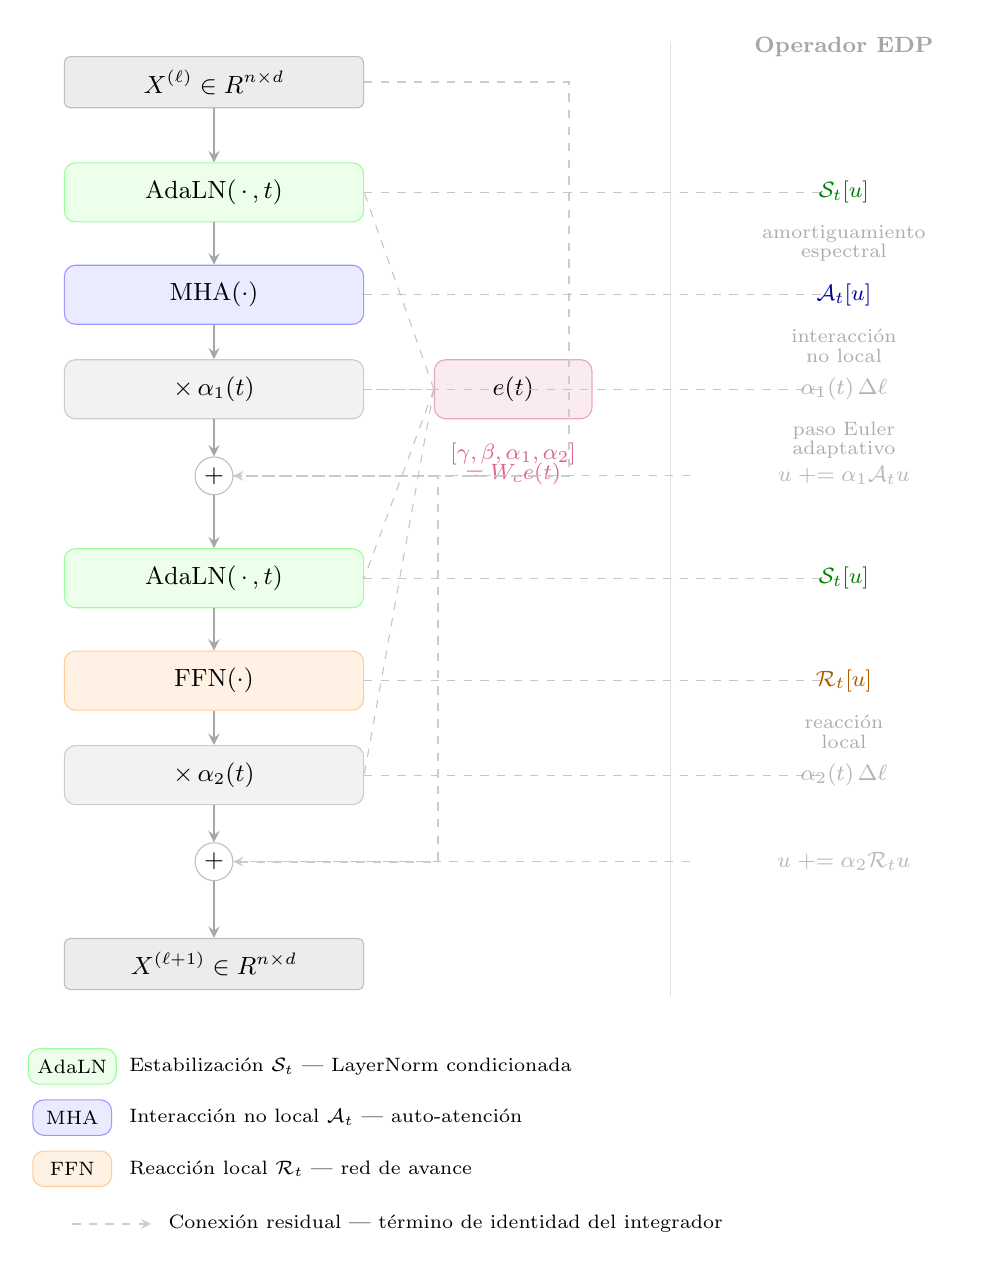
\begin{tikzpicture}[
  % ── estilos de nodos ──────────────────────────────────────
  block/.style={
    rectangle, rounded corners=4pt,
    minimum width=3.8cm, minimum height=0.75cm,
    text centered, font=\small,
    draw=gray!60, line width=0.4pt
  },
  blockA/.style={block,
    fill=blue!8,  draw=blue!40},   % atención
  blockR/.style={block,
    fill=orange!10, draw=orange!40}, % FFN / reacción
  blockS/.style={block,
    fill=green!8, draw=green!40},  % AdaLN / estabilización
  blockG/.style={block,
    fill=gray!10, draw=gray!40},   % gate / escalar
  io/.style={
    rectangle, rounded corners=2pt,
    minimum width=3.8cm, minimum height=0.65cm,
    text centered, font=\small\itshape,
    fill=gray!15, draw=gray!50, line width=0.4pt
  },
  % ── anotaciones EDP ───────────────────────────────────────
  edpbox/.style={
    rectangle, rounded corners=3pt,
    minimum width=3.4cm, minimum height=0.65cm,
    text centered, font=\footnotesize,
    draw=none, fill=none
  },
  % ── flechas ───────────────────────────────────────────────
  arr/.style={-stealth, gray!70, line width=0.8pt},
  arrres/.style={-stealth, gray!40, line width=0.6pt,
                 dashed},          % conexión residual
  leader/.style={gray!45, line width=0.4pt, dashed}
]

% ════════════════════════════════════════════════════════════
%  COLUMNA IZQUIERDA — flujo arquitectónico
% ════════════════════════════════════════════════════════════

\def\cx{0}      % centro de la columna de bloques
\def\cxr{2.4}   % punto de salida de la conexión residual

% -- Input ------------------------------------------------
\node[io] (in) at (\cx, 0)
  {$\bm{X}^{(\ell)} \in \mathbb{R}^{n \times d}$};

% -- AdaLN 1 (pre-norm, atención) -------------------------
\node[blockS] (ln1) at (\cx, -1.4)
  {$\mathrm{AdaLN}(\,\cdot\,,t)$};

% -- MHA --------------------------------------------------
\node[blockA] (mha) at (\cx, -2.7)
  {$\mathrm{MHA}(\cdot)$};

% -- Gate alpha_1 -----------------------------------------
\node[blockG] (g1) at (\cx, -3.9)
  {$\times\,\alpha_1(t)$};

% -- Suma residual 1 (nodo explícito) ---------------------
\node[circle, draw=gray!50, fill=white,
      inner sep=1.5pt, font=\small] (sum1) at (\cx, -5.0)
  {$+$};

% -- AdaLN 2 (pre-norm, FFN) ------------------------------
\node[blockS] (ln2) at (\cx, -6.3)
  {$\mathrm{AdaLN}(\,\cdot\,,t)$};

% -- FFN --------------------------------------------------
\node[blockR] (ffn) at (\cx, -7.6)
  {$\mathrm{FFN}(\cdot)$};

% -- Gate alpha_2 -----------------------------------------
\node[blockG] (g2) at (\cx, -8.8)
  {$\times\,\alpha_2(t)$};

% -- Suma residual 2 --------------------------------------
\node[circle, draw=gray!50, fill=white,
      inner sep=1.5pt, font=\small] (sum2) at (\cx, -9.9)
  {$+$};

% -- Output -----------------------------------------------
\node[io] (out) at (\cx, -11.2)
  {$\bm{X}^{(\ell+1)} \in \mathbb{R}^{n \times d}$};

% -- Embedding de tiempo (lateral) ------------------------
\node[block, fill=purple!8, draw=purple!35,
      minimum width=2.0cm, font=\small]
  (emb) at (3.8, -3.9)
  {$\bm{e}(t)$};

\node[font=\footnotesize, text=purple!60, align=center]
  at (3.8, -4.85)
  {$[\gamma,\beta,\alpha_1,\alpha_2]$\\[-2pt]$=\bm{W}_c\bm{e}(t)$};

% ── flechas principales ───────────────────────────────────
\draw[arr] (in)   -- (ln1);
\draw[arr] (ln1)  -- (mha);
\draw[arr] (mha)  -- (g1);
\draw[arr] (g1)   -- (sum1);
\draw[arr] (sum1) -- (ln2);
\draw[arr] (ln2)  -- (ffn);
\draw[arr] (ffn)  -- (g2);
\draw[arr] (g2)   -- (sum2);
\draw[arr] (sum2) -- (out);

% ── conexiones residuales (bypass) ────────────────────────
% residual 1: in -> sum1
\draw[arrres]
  (in.east) -- ++({\cxr - \cx + 0.2}, 0)
  -- ++(0, {-5.0 + 0.0})
  -- (sum1.east);

% residual 2: sum1 -> sum2
\draw[arrres]
  (sum1.east) -- ++({\cxr - \cx + 0.2}, 0)
  -- ++(0, {-4.9})
  -- (sum2.east);

% ── embedding conectado a AdaLN y gates ──────────────────
\draw[leader] (emb.west) -- (ln1.east);
\draw[leader] (emb.west) -- (ln2.east);
\draw[leader] (emb.west) -- (g1.east);
\draw[leader] (emb.west) -- (g2.east);

% ════════════════════════════════════════════════════════════
%  COLUMNA DERECHA — anotaciones EDP
% ════════════════════════════════════════════════════════════

\def\ex{8.0}   % x de las etiquetas EDP

% separador vertical
\draw[gray!25, line width=0.5pt] (5.8, 0.5) -- (5.8, -11.6);

\node[font=\footnotesize\bfseries, gray!70]
  at (\ex, 0.45) {Operador EDP};

% -- AdaLN <-> S ------------------------------------------
\draw[leader] (ln1.east) -- ++({(\ex - \cx - 1.9 - 0.2)}, 0);
\node[edpbox, text=green!50!black] at (\ex, -1.4)
  {$\mathcal{S}_t[\bm{u}]$};
\node[font=\scriptsize, text=gray!65, align=center]
  at (\ex, -2.05)
  {amortiguamiento\\[-1pt]espectral};

% -- MHA <-> A --------------------------------------------
\draw[leader] (mha.east) -- ++({(\ex - \cx - 1.9 - 0.2)}, 0);
\node[edpbox, text=blue!60!black] at (\ex, -2.7)
  {$\mathcal{A}_t[\bm{u}]$};
\node[font=\scriptsize, text=gray!65, align=center]
  at (\ex, -3.35)
  {interacción\\[-1pt]no local};

% -- Gate <-> coef. Euler ---------------------------------
\draw[leader] (g1.east) -- ++({(\ex - \cx - 1.9 - 0.2)}, 0);
\node[edpbox, text=gray!60] at (\ex, -3.9)
  {$\alpha_1(t)\,\Delta\ell$};
\node[font=\scriptsize, text=gray!65, align=center]
  at (\ex, -4.55)
  {paso Euler\\[-1pt]adaptativo};

% -- sum1 <-> discretización Euler ------------------------
\draw[leader] (sum1.east) -- ++({(\ex - \cx - 1.9 - 0.2)}, 0);
\node[edpbox, text=gray!55] at (\ex, -5.0)
  {$\bm{u} \mathrel{+}= \alpha_1\mathcal{A}_t\bm{u}$};

% -- AdaLN 2 <-> S ----------------------------------------
\draw[leader] (ln2.east) -- ++({(\ex - \cx - 1.9 - 0.2)}, 0);
\node[edpbox, text=green!50!black] at (\ex, -6.3)
  {$\mathcal{S}_t[\bm{u}]$};

% -- FFN <-> R --------------------------------------------
\draw[leader] (ffn.east) -- ++({(\ex - \cx - 1.9 - 0.2)}, 0);
\node[edpbox, text=orange!70!black] at (\ex, -7.6)
  {$\mathcal{R}_t[\bm{u}]$};
\node[font=\scriptsize, text=gray!65, align=center]
  at (\ex, -8.25)
  {reacción\\[-1pt]local};

% -- Gate 2 -----------------------------------------------
\draw[leader] (g2.east) -- ++({(\ex - \cx - 1.9 - 0.2)}, 0);
\node[edpbox, text=gray!60] at (\ex, -8.8)
  {$\alpha_2(t)\,\Delta\ell$};

% -- sum2 -------------------------------------------------
\draw[leader] (sum2.east) -- ++({(\ex - \cx - 1.9 - 0.2)}, 0);
\node[edpbox, text=gray!55] at (\ex, -9.9)
  {$\bm{u} \mathrel{+}= \alpha_2\mathcal{R}_t\bm{u}$};

% ════════════════════════════════════════════════════════════
%  LEYENDA
% ════════════════════════════════════════════════════════════

\begin{scope}[shift={(-1.8, -12.5)}]
  \node[blockS, minimum width=1.0cm, minimum height=0.45cm,
        font=\scriptsize] at (0,0)     {AdaLN};
  \node[font=\scriptsize, anchor=west] at (0.6, 0)
    {Estabilización $\mathcal{S}_t$ — LayerNorm condicionada};

  \node[blockA, minimum width=1.0cm, minimum height=0.45cm,
        font=\scriptsize] at (0,-0.65) {MHA};
  \node[font=\scriptsize, anchor=west] at (0.6,-0.65)
    {Interacción no local $\mathcal{A}_t$ — auto-atención};

  \node[blockR, minimum width=1.0cm, minimum height=0.45cm,
        font=\scriptsize] at (0,-1.3) {FFN};
  \node[font=\scriptsize, anchor=west] at (0.6,-1.3)
    {Reacción local $\mathcal{R}_t$ — red de avance};

  \draw[arrres] (0,-2.0) -- (1.0,-2.0);
  \node[font=\scriptsize, anchor=west] at (1.1,-2.0)
    {Conexión residual — término de identidad del integrador};
\end{scope}

\end{tikzpicture}

\caption{Arquitectura del bloque DiT y su correspondencia con los
operadores de la EDP maestra~\eqref{eq:master_pde_t}.
\textbf{Izquierda:} flujo de datos a través del bloque.
El embedding de tiempo $\bm{e}(t)$ (morado) genera simultáneamente
los parámetros de AdaLN ($\gamma, \beta$) y los gates adaptativos
($\alpha_1, \alpha_2$) para todas las capas.
Las líneas discontinuas representan las conexiones residuales
que implementan el término de identidad del integrador de Euler.
\textbf{Derecha:} operador de la EDP maestra~\eqref{eq:master_pde_t}
al que corresponde cada componente. La evolución discreta capa a capa
$\bm{u}^{(\ell+1)} = \bm{u}^{(\ell)}
+ \alpha_1(t)\mathcal{A}_t[\bm{u}^{(\ell)}]
+ \alpha_2(t)\mathcal{R}_t[\bm{u}^{(\ell)}]$
es el método de Euler aplicado a la EDP continua
$\partial_\ell \bm{u} = \mathcal{A}_t[\bm{u}] + \mathcal{R}_t[\bm{u}]$.}
\label{fig:dit_bloque}
\end{figure}

%────────────────────────────────────────────────────────────────
\section{Redes equivariantes de grupo: el caso SO(3)}
\label{sec:so3}
\dificultad{4}{3}
%────────────────────────────────────────────────────────────────

Esta sección desarrolla la forma canónica de las capas equivariantes
para el grupo de rotaciones $\mathrm{SO}(3)$. Requiere familiaridad
con la teoría de representaciones de grupos de Lie: armónicos
esféricos, matrices de Wigner y coeficientes de Clebsch-Gordan.
Un físico de partículas o de estructura nuclear reconocerá estos
objetos desde la mecánica cuántica del momento angular; un lector
sin ese background puede continuar al Capítulo~\ref{ch:cap10} sin
pérdida de continuidad. Las arquitecturas de difusión de los
Capítulos~\ref{ch:cap11}--\ref{ch:cap12} no dependen de esta sección.

\subsubsection*{Armónicos esféricos como base de las representaciones}

Los armónicos esféricos $Y_l^m: S^2 \to \mathbb{C}$ son las autofunciones del
operador de Laplace-Beltrami en la esfera $S^2$:
\[
  \nabla^2_{S^2} Y_l^m = -l(l+1)Y_l^m.
\]
Son ortogonales: $\int_{S^2} Y_l^m(\hat{\bm{r}})\overline{Y_{l'}^{m'}(\hat{\bm{r}})}\,
d\hat{\bm{r}} = \delta_{ll'}\delta_{mm'}$, y completos en $L^2(S^2)$.

Bajo una rotación $R \in \mathrm{SO}(3)$, los armónicos esféricos de grado $l$
transforman entre sí mediante la \textbf{matriz de Wigner} $\bm{D}^l(R)$:
\begin{equation}
  Y_l^m(R^{-1}\hat{\bm{r}}) = \sum_{m'=-l}^l D_{m'm}^l(R)\,Y_l^{m'}(\hat{\bm{r}}).
  \label{eq:wigner}
\end{equation}
Las matrices de Wigner $\bm{D}^l(R) \in \mathbb{C}^{(2l+1)\times(2l+1)}$
son exactamente las representaciones irreducibles de $\mathrm{SO}(3)$:
$\bm{D}^l: \mathrm{SO}(3) \to \mathrm{GL}(\mathbb{C}^{2l+1})$.

Para aplicaciones físicas reales se usan versiones reales $Y_l^m$ (combinaciones
lineales de las complejas), con matrices de Wigner reales correspondientes.

Los primeros armónicos (reales):
\begin{align*}
  l=0:&\quad Y_0^0 = \frac{1}{\sqrt{4\pi}} \quad (\text{invariante bajo rotaciones}) \\
  l=1:&\quad Y_1^{-1} \propto y/r,\; Y_1^0 \propto z/r,\; Y_1^1 \propto x/r
        \quad (\text{componentes de un vector}) \\
  l=2:&\quad \text{cinco componentes de un tensor simétrico sin traza.}
\end{align*}

\begin{fisicaconexion}{Armónicos esféricos en física atómica y electromagnetismo}
Los armónicos esféricos son ubicuos en física porque $\mathrm{SO}(3)$ es el
grupo de simetría de cualquier problema con simetría esférica. En
\textbf{mecánica cuántica}, los orbitales atómicos del hidrógeno son
$\psi_{nlm}(r,\theta,\phi) = R_{nl}(r)\,Y_l^m(\theta,\phi)$, donde $l$ es el
número cuántico de momento angular y $m$ el magnético. Los estados $s$, $p$,
$d$, $f$ corresponden a $l = 0, 1, 2, 3$: exactamente los primeros irreducibles
de $\mathrm{SO}(3)$. Las reglas de selección de las transiciones atómicas
($\Delta l = \pm 1$, $\Delta m = 0, \pm 1$) son las reglas de Clebsch-Gordan
del producto $V_l \otimes V_1$ (fotón de espín 1): solo los $l$ que aparecen
en la descomposición~\eqref{eq:cg_decomp} están permitidos.

En \textbf{electromagnetismo}, la expansión multipolar del potencial de una
distribución de carga a distancia $r \gg r'$ es:
\[
  \phi(\bm{r}) = \frac{1}{4\pi\epsilon_0}\sum_{l=0}^\infty \sum_{m=-l}^l
  \frac{4\pi}{2l+1}\,q_{lm}\,\frac{Y_l^m(\hat{\bm{r}})}{r^{l+1}},
\]
donde $q_{lm} = \int r'^l Y_l^{m*}(\hat{\bm{r}}')\rho(\bm{r}')d\bm{r}'$ son
los \textbf{momentos multipolares}: escalar ($l=0$), dipolo ($l=1$), cuadrupolo
($l=2$), etc. Los mismos $l$ que clasifican los irreducibles de $\mathrm{SO}(3)$
indexan los multipolos. En RMN, las matrices de Wigner $\bm{D}^l(R)$
aparecen al describir cómo los tensores de desplazamiento químico y acoplamiento
dipolar transforman bajo rotaciones de la muestra en experimentos de ángulo
mágico. La ecuación~\eqref{eq:wigner} no es solo una fórmula de redes neuronales:
es la ley de transformación de cualquier objeto tensorial de rango $l$ bajo
rotaciones.
\end{fisicaconexion}
\label{subsec:cg}

El producto tensorial de dos representaciones irreducibles de $\mathrm{SO}(3)$
de órdenes $l_1$ y $l_2$ se descompone en suma directa de irreducibles:
\begin{equation}
  V_{l_1} \otimes V_{l_2} \cong \bigoplus_{l=|l_1-l_2|}^{l_1+l_2} V_l.
  \label{eq:cg_decomp}
\end{equation}
Esta descomposición es la \textbf{regla de selección de Clebsch-Gordan}.
Los vectores de la base del irreducible $V_l$ en el producto $V_{l_1}\otimes V_{l_2}$
son:
\begin{equation}
  |l, m\rangle = \sum_{m_1=-l_1}^{l_1} \sum_{m_2=-l_2}^{l_2}
  C_{m_1 m_2 m}^{l_1 l_2 l}\,|l_1, m_1\rangle \otimes |l_2, m_2\rangle,
  \label{eq:cg_vector}
\end{equation}
donde $C_{m_1 m_2 m}^{l_1 l_2 l}$ son los \textbf{coeficientes de Clebsch-Gordan}.
Son cero a menos que $m = m_1+m_2$ y $|l_1-l_2| \leq l \leq l_1+l_2$.

En notación de operador, la proyección del producto tensorial sobre el irreducible
$V_l$ define el \textbf{producto tensorial de Clebsch-Gordan}:
\[
  (\bm{f}^{l_1} \otimes_{CG}^l \bm{g}^{l_2})_m
  = \sum_{m_1, m_2} C_{m_1 m_2 m}^{l_1 l_2 l}\,
  f_{m_1}^{l_1}\,g_{m_2}^{l_2}.
\]

\subsection{La capa equivariante bajo SO(3): derivación completa}
\label{subsec:so3_layer}

Una capa equivariante bajo $\mathrm{SO}(3)$ mapea
$\bm{f} = \bigoplus_{l_{\mathrm{in}}} \bm{f}^{l_{\mathrm{in}}}$ a
$\bm{h} = \bigoplus_{l_{\mathrm{out}}} \bm{h}^{l_{\mathrm{out}}}$,
donde $\bm{f}^{l_{\mathrm{in}}} \in \mathbb{R}^{(2l_{\mathrm{in}}+1)\times C_{l_{\mathrm{in}}}}$
son las características del tipo $l_{\mathrm{in}}$ (con $C_{l_{\mathrm{in}}}$
canales) y análogamente para la salida.

\begin{teorema}{Forma canónica de la capa equivariante bajo SO(3)}
\label{thm:so3_layer}
La capa lineal más general que es equivariante bajo $\mathrm{SO}(3)$ tiene la
forma:
\begin{equation}
  h_{m_{\mathrm{out}}, c_{\mathrm{out}}}^{l_{\mathrm{out}}}
  = \sum_{l_{\mathrm{in}}, l_f} \sum_{m_{\mathrm{in}}, m_f}
  \sum_{c_{\mathrm{in}}}
  C_{m_{\mathrm{in}} m_f m_{\mathrm{out}}}^{l_{\mathrm{in}} l_f l_{\mathrm{out}}}
  \cdot w_{c_{\mathrm{in}} c_{\mathrm{out}}}^{l_{\mathrm{in}} l_f l_{\mathrm{out}}}
  \cdot f_{m_{\mathrm{in}}, c_{\mathrm{in}}}^{l_{\mathrm{in}}}
  \cdot Y_{l_f}^{m_f}(\hat{\bm{r}}),
  \label{eq:so3_layer}
\end{equation}
donde $\hat{\bm{r}}$ es la dirección de una arista (en grafos moleculares),
$Y_{l_f}^{m_f}$ son los armónicos esféricos del edge, y $w_{c_{\mathrm{in}}
c_{\mathrm{out}}}^{l_{\mathrm{in}} l_f l_{\mathrm{out}}} \in \mathbb{R}$ son
los únicos parámetros libres aprendibles.
\end{teorema}

\begin{proof}
Por el Lema de Schur, $\bm{W}$ es equivariante si y solo si, en la
descomposición en irreducibles, solo conecta irreducibles del mismo tipo.
La representación de entrada en el nodo es $\bigoplus_{l_{\mathrm{in}}}
\bm{D}^{l_{\mathrm{in}}}$. Los armónicos esféricos de la arista transforman
como $\bigoplus_{l_f} \bm{D}^{l_f}$. El producto tensorial de la
característica de entrada y el armónico de la arista es:
\[
  V_{l_{\mathrm{in}}} \otimes V_{l_f}
  \cong \bigoplus_{l=|l_{\mathrm{in}}-l_f|}^{l_{\mathrm{in}}+l_f} V_l.
\]
Para conectar este producto con la salida $V_{l_{\mathrm{out}}}$, por el
Lema de Schur solo es posible si $l_{\mathrm{out}}$ aparece en la
descomposición, es decir $|l_{\mathrm{in}}-l_f| \leq l_{\mathrm{out}}
\leq l_{\mathrm{in}}+l_f$ (regla de selección de Clebsch-Gordan).
Dentro de cada bloque permitido, el Lema de Schur establece que el único
mapa lineal equivariante es un múltiplo escalar de la identidad en ese bloque:
ese escalar es exactamente $w_{c_{\mathrm{in}} c_{\mathrm{out}}}^{l_{\mathrm{in}}
l_f l_{\mathrm{out}}}$, con un grado de libertad por cada tripleta
$(l_{\mathrm{in}}, l_f, l_{\mathrm{out}})$ y par de canales $(c_{\mathrm{in}},
c_{\mathrm{out}})$ que satisfaga la regla de selección. El mapa explícito es
el producto de Clebsch-Gordan de~\eqref{eq:so3_layer}. $\square$
\end{proof}

\begin{observacion}{Conteo de parámetros equivariantes}
Para tipos de orden máximo $l_{\max}$, el número de tipos de irreducibles es
$l_{\max}+1$ y el número de tripletas permitidas $(l_{\mathrm{in}}, l_f,
l_{\mathrm{out}})$ es $O(l_{\max}^3)$. Los parámetros aprendibles son escalares:
el costo de la capa es $O(l_{\max}^3 C^2)$ parámetros (con $C$ canales por
tipo), significativamente menor que el costo de una capa densa no equivariante
de la misma dimensión, que sería $O((l_{\max}C)^2 (2l_{\max}+1)^2)$.
\end{observacion}

\subsection{Ejemplos de arquitecturas SO(3)-equivariantes}
\label{subsec:so3_arqs}

La estructura de la ecuación~\eqref{eq:so3_layer} aparece en múltiples
arquitecturas para datos 3D:

\medskip
\noindent\textbf{e3nn} (Geiger y Smidt, 2022): implementación modular de capas
equivariantes para cualquier grupo $O(3)$. Los tipos son \textit{scalars}
($l=0$), \textit{vectors} ($l=1$), \textit{tensors} ($l=2$, etc.).

\medskip
\noindent\textbf{NequIP/MACE} (Batzner et al., 2022; Batatia et al., 2022):
para potenciales interatómicos de aprendizaje automático. Las características
de los nodos son tensores esféricos de los átomos; las interacciones entre
pares de átomos se convoluciona con los armónicos esféricos de la dirección
interatómica. El resultado respeta exactamente las simetrías de traslación,
rotación y reflexión de la mecánica molecular.

\subsection{Construcción sistemática para grupos generales}
\label{subsec:grupo_general}

El procedimiento general para construir una capa equivariante bajo un grupo
compacto $G$ dado es:
\begin{enumerate}
  \item Calcular la tabla de caracteres de $G$: las trazas
        $\chi^\alpha(g) = \mathrm{tr}(\rho^\alpha(g))$ de cada clase de
        conjugación para cada irreducible $\rho^\alpha$.
  \item Descomponer las representaciones de entrada y salida en irreducibles
        usando las relaciones de ortogonalidad:
        $m_\alpha = \frac{1}{|G|}\sum_g \chi^\alpha(g^{-1})\chi_{\mathrm{in}}(g)$.
  \item Por el Lema de Schur, los únicos pesos libres son escalares que
        multiplican el mapa identidad en cada bloque de irreducibles equivalentes.
\end{enumerate}
Este procedimiento es completamente algorítmico y se implementa para cualquier
grupo finito o de Lie compacto.

%───────────────────────────────────────────────────────────────────────────────
\section{Conexiones residuales y Neural ODEs}
\label{sec:resnet_node}
\dificultad{3}{3}
%───────────────────────────────────────────────────────────────────────────────

\subsection{El problema del gradiente en redes profundas}
\label{subsec:grad_profundo}

Para un MLP de $L$ capas, el error de la capa $l$ es:
\[
  \bm{\delta}^{(l)}
  = \Biggl(\prod_{k=l+1}^L \bm{W}^{(k)\top}
    \mathrm{diag}(\sigma'^{(k)}(\bm{z}^{(k)}))\Biggr)\bm{\delta}^{(L)}.
\]
Si las normas espectrales de los jacobianos son en promedio $< 1$, el gradiente
se desvanece exponencialmente en $L-l$. Si son $> 1$, explota. Para $L = 100$
capas, incluso una norma media de $0.99$ da $0.99^{100} \approx 0.37$:
el gradiente llega a la primera capa con $37\%$ de su magnitud original,
lo que es manejable; pero una norma de $0.9$ da $0.9^{100} \approx 3\times 10^{-5}$:
el gradiente prácticamente desaparece.

\subsection{Las conexiones residuales como integrador de Euler}
\label{subsec:residual}

\begin{definicion}{Bloque residual}
\label{def:residual}
Un \textbf{bloque residual} (\textit{residual block}) es:
\[
  \bm{a}^{(l+1)} = \bm{a}^{(l)} + F(\bm{a}^{(l)};\bm{\theta}^{(l)}),
\]
donde $F$ es típicamente una secuencia de dos capas con normalización y
activación, y $\bm{a}^{(l)}$ y $F$ tienen la misma dimensión.
\end{definicion}

El backward pass de la conexión residual:
\[
  \bm{\delta}^{(l)} = \frac{\partial\mathcal{L}}{\partial\bm{a}^{(l)}}
  = \frac{\partial\mathcal{L}}{\partial\bm{a}^{(l+1)}}
  \cdot\left(\bm{I} + \frac{\partial F}{\partial\bm{a}^{(l)}}\right)
  = \bm{\delta}^{(l+1)}\left(\bm{I} + \bm{J}_F^{(l)}\right).
\]
El término identidad garantiza que el gradiente $\bm{\delta}^{(l+1)}$ llega
intacto a la capa $l$, independientemente de la magnitud de $\bm{J}_F^{(l)}$.
Para redes con $L = 100$--$1000$ bloques residuales, este mecanismo hace el
entrenamiento estable.

La interpretación como integrador: la ecuación
$\bm{a}^{(l+1)} = \bm{a}^{(l)} + F(\bm{a}^{(l)})$ es el método de Euler
con paso $h = 1$ para la ODE:
\[
  \frac{d\bm{a}}{dt} = F(\bm{a}(t);\bm{\theta}),
  \qquad \bm{a}(0) = \bm{a}^{(0)},
\]
con $\bm{a}^{(l)} = \bm{a}(l)$. La profundidad $L$ es el número de pasos
de Euler; la activación de la última capa es $\bm{a}(L)$, la solución
aproximada de la ODE.

\subsection{Neural ODEs: profundidad continua y el método adjunto completo}
\label{subsec:neural_ode}

La \textbf{Neural ODE} (Chen et al., 2018) toma este límite en serio: en lugar
de discretizar con $L$ pasos de Euler, usa un integrador numérico de alta
precisión para resolver la ODE exacta:
\begin{equation}
  \frac{d\bm{a}(t)}{dt} = F(\bm{a}(t), t;\bm{\theta}),
  \qquad \bm{a}(t_0) = \bm{a}^{(0)},
  \label{eq:neural_ode}
\end{equation}
y la predicción es $\hat{\bm{y}} = g(\bm{a}(t_1))$ donde $g$ es una capa de
salida. El forward pass es la integración numérica de~\eqref{eq:neural_ode}
de $t_0$ a $t_1$.

El problema del backward pass es calcular $\nabla_{\bm{\theta}}\mathcal{L}$
donde $\mathcal{L} = \ell(\hat{\bm{y}}, \bm{y}) = \ell(g(\bm{a}(t_1)),\bm{y})$.
La solución naïve (backpropagation a través de los pasos del integrador) requiere
almacenar todas las activaciones intermedias del integrador: para un integrador
de orden 4 con $N_{\text{steps}}$ pasos, esto es $O(N_{\text{steps}})$ en memoria.
La Neural ODE resuelve esto con el \textbf{método adjunto}, reduciendo el costo
de memoria a $O(1)$.

\subsubsection*{Derivación completa del método adjunto para Neural ODEs}

Se considera el problema general de minimizar $\mathcal{L} = \int_{t_0}^{t_1}
r(\bm{a}(t),\bm{\theta},t)\,dt + \ell(\bm{a}(t_1),\bm{y})$ sujeto a~\eqref{eq:neural_ode}.
Para la Neural ODE estándar $r = 0$.

\medskip
\noindent\textbf{Paso 1: el estado adjunto.}
Se define el \textbf{estado adjunto} (o co-estado):
\begin{equation}
  \bm{\lambda}(t) = \frac{d\mathcal{L}}{d\bm{a}(t)} \in \mathbb{R}^d.
  \label{eq:adjunto_def}
\end{equation}
La condición terminal es $\bm{\lambda}(t_1) = \frac{d\ell}{d\bm{a}(t_1)}
= \nabla_{\bm{a}(t_1)}\ell$.

\medskip
\noindent\textbf{Paso 2: la ecuación adjunta.}
Se calcula $d\bm{\lambda}/dt$ usando la fórmula de Itô para el funcional
continuo (o equivalentemente, diferenciando la identidad de sensibilidad).
Para un incremento $\delta t$, la variación $\delta\bm{a}(t)$ se propaga
según la ecuación variacional:
\[
  \frac{d}{dt}\delta\bm{a}(t)
  = \frac{\partial F(\bm{a}(t),t;\bm{\theta})}{\partial\bm{a}}\delta\bm{a}(t)
  = \bm{J}_F(t)\,\delta\bm{a}(t).
\]
La variación de la pérdida es:
\[
  \delta\mathcal{L} = \bm{\lambda}(t_1)^\top\delta\bm{a}(t_1)
  = \bm{\lambda}(t_1)^\top
  \underbrace{\left[\bm{I} + \int_t^{t_1}\bm{J}_F(s)\,ds + O(\Delta t^2)\right]}
  _{\text{propagador linealizado}}
  \delta\bm{a}(t).
\]
Diferenciando respecto a $t$:
\[
  \frac{d\bm{\lambda}(t)^\top}{dt}
  = -\bm{\lambda}(t)^\top\bm{J}_F(t),
\]
es decir:
\begin{equation}
  \frac{d\bm{\lambda}}{dt}
  = -\bm{J}_F(t)^\top\bm{\lambda}(t)
  = -\left(\frac{\partial F(\bm{a}(t),t;\bm{\theta})}{\partial\bm{a}}\right)^\top
  \bm{\lambda}(t).
  \label{eq:adj_ode}
\end{equation}
Esta es la \textbf{ecuación adjunta}: una ODE lineal no autónoma para
$\bm{\lambda}(t)$ que se integra \textbf{hacia atrás} desde $t_1$ hasta $t_0$.

\medskip
\noindent\textbf{Paso 3: el gradiente respecto a los parámetros.}
La variación de $\mathcal{L}$ respecto a un cambio $\delta\bm{\theta}$ en los
parámetros es, usando la fórmula de sensibilidad paramétrica:
\begin{equation}
  \frac{d\mathcal{L}}{d\bm{\theta}}
  = \int_{t_0}^{t_1}
  \bm{\lambda}(t)^\top
  \frac{\partial F(\bm{a}(t),t;\bm{\theta})}{\partial\bm{\theta}}\,dt.
  \label{eq:grad_theta}
\end{equation}

\medskip
\noindent\textbf{Paso 4: el algoritmo adjunto completo.}
El Algoritmo~\ref{alg:adj_ode} resume el procedimiento.

\begin{algorithm}[H]
\caption{Método adjunto para Neural ODEs}
\label{alg:adj_ode}
\KwIn{Red $F(\cdot,\cdot;\bm{\theta})$, pérdida $\ell$, entrada $\bm{a}^{(0)}$,
      intervalo $[t_0,t_1]$}
\KwOut{$\mathcal{L}$, $\nabla_{\bm{a}^{(0)}}\mathcal{L}$,
       $\nabla_{\bm{\theta}}\mathcal{L}$}

\tcp{--- Forward pass: integrar la Neural ODE ---}
$\bm{a}(t_1) \leftarrow \mathrm{ODESolve}\!\left(F,\,\bm{a}(t_0),\,[t_0,t_1]\right)$\;
$\mathcal{L} \leftarrow \ell(\bm{a}(t_1),\bm{y})$\;

\tcp{--- Inicializar el estado adjunto ---}
$\bm{\lambda}(t_1) \leftarrow \nabla_{\bm{a}(t_1)}\ell$\;
$\bm{a}_{\bm{\theta}}(t_1) \leftarrow \bm{0}$ \tcp*{acumulador del gradiente}

\tcp{--- Backward pass: integrar la ecuación adjunta hacia atrás ---}
$\begin{pmatrix}\bm{a}(t_0)\\\bm{\lambda}(t_0)\\\nabla_{\bm{\theta}}\mathcal{L}\end{pmatrix}
\leftarrow
\mathrm{ODESolve}\!\left(
  \begin{pmatrix}
    F(\bm{a},t;\bm{\theta})\\
    -\bm{J}_F^\top\bm{\lambda}\\
    -\bm{\lambda}^\top\partial_{\bm{\theta}}F
  \end{pmatrix},\;
  \begin{pmatrix}\bm{a}(t_1)\\\bm{\lambda}(t_1)\\\bm{0}\end{pmatrix},\;
  [t_1,t_0]\right)$\;

\Return $\mathcal{L}$, $\bm{\lambda}(t_0)$,
        $\nabla_{\bm{\theta}}\mathcal{L}$\;
\end{algorithm}

\subsubsection*{Correspondencia con el principio de Pontryagin}

La conexión con el formalismo del Capítulo~\ref{ch:cap6} es exacta. Identificando:
\begin{center}
\begin{tabular}{ll}
\toprule
\textbf{Neural ODE} & \textbf{MLP (Cap.~\ref{ch:cap6})} \\
\midrule
Estado $\bm{a}(t)$ & Post-activación $\bm{a}^{(l)}$ \\
Control $\bm{\theta}$ & Parámetros $(\bm{W}^{(l)},\bm{b}^{(l)})$ \\
ODE $\dot{\bm{a}} = F(\bm{a},t;\bm{\theta})$ & Forward pass discreto \\
Co-estado $\bm{\lambda}(t)$ & Error $\bm{\delta}^{(l)} = -\bm{\lambda}^{(l)}$ \\
Ec.\ adjunta $\dot{\bm{\lambda}} = -\bm{J}_F^\top\bm{\lambda}$ & BP2 continua \\
Condición terminal $\bm{\lambda}(t_1) = \nabla\ell$ & BP1 \\
Gradiente $\int\bm{\lambda}^\top\partial_{\bm{\theta}}F\,dt$ & BP3 acumulado \\
\bottomrule
\end{tabular}
\end{center}

El MLP del Capítulo~\ref{ch:cap4} es una Neural ODE discretizada con el método de Euler.
El método adjunto del Capítulo~\ref{ch:cap6} es la discretización del Algoritmo~\ref{alg:adj_ode}.
El principio de Pontryagin es el caso continuo de backpropagation.

\subsubsection*{Ventajas y costo del método adjunto}

\medskip
\noindent\textbf{Memoria $O(1)$:} el backward pass no requiere almacenar las
activaciones intermedias del forward pass: las recomputa integrando la ODE
del estado hacia atrás en paralelo con la ecuación adjunta. El costo de memoria
es $O(d + p)$ (estado más parámetros), independiente del número de pasos del
integrador.

\medskip
\noindent\textbf{Costo computacional:} el backward pass requiere integrar
numéricamente el sistema aumentado de dimensión $2d + p$ en lugar de $d$.
El costo es $\sim 3\times$ el del forward pass, idéntico al de backpropagation
estándar.

\medskip
\noindent\textbf{Precisión adaptativa:} el integrador del backward pass puede
elegir el paso adaptativo para controlar el error numérico de la ecuación
adjunta. En backpropagation estándar, el error numérico se acumula fijo capa
a capa.

\begin{fisicaconexion}{Ecuaciones diferenciales en física y el método adjunto en control óptimo}
La Neural ODE~\eqref{eq:neural_ode} es formalmente idéntica a la ecuación de
movimiento de un sistema dinámico con estado $\bm{a}(t)$ y campo de fuerza
$F(\bm{a},t;\bm{\theta})$. Para un oscilador anarmónico $\ddot{x} = -\omega^2 x -
\epsilon x^3$, la ecuación de segundo orden se escribe como sistema de primer
orden $\dot{\bm{a}} = (a_2, -\omega^2 a_1 - \epsilon a_1^3)$: exactamente la
forma de~\eqref{eq:neural_ode}, con $F$ determinado por la física en lugar de
aprendido.

El método adjunto del Algoritmo~\ref{alg:adj_ode} es la forma continua del
\textbf{principio del mínimo de Pontryagin} en teoría de control óptimo. El
problema clásico de control de trayectoria de un cohete o satélite es:
minimizar el combustible consumido $\mathcal{L} = \int_0^T \|\bm{u}(t)\|^2\,dt$
sujeto a la dinámica $\dot{\bm{x}} = f(\bm{x},\bm{u})$ (ecuación del
movimiento), con condición final $\bm{x}(T) = \bm{x}_f$ (destino). El método
adjunto introduce el \textbf{co-estado} $\bm{p}(t)$ (el vector de multiplicadores
de Lagrange en el tiempo) que satisface exactamente la ecuación adjunta
$\dot{\bm{p}} = -(\partial f/\partial \bm{x})^\top\bm{p}$: la misma
ecuación~\eqref{eq:adj_ode}. El control óptimo es $\bm{u}^*(t) = -\bm{p}(t)/2$
(para este caso cuadrático), obtenido sin integrar la dinámica en sentido
inverso.

En \textbf{óptica geométrica}, la ecuación eikonal $|\nabla S| = n(\bm{r})$
(con $S$ el frente de onda y $n$ el índice de refracción) tiene la misma
estructura: los rayos de luz son trayectorias del sistema hamiltoniano
$\dot{\bm{q}} = \bm{p}/n$, $\dot{\bm{p}} = \nabla n$. El estado adjunto de un
problema de diseño de lentes (minimizar aberración sujeto a la propagación de
rayos) es exactamente el vector de sensibilidad del frente de onda respecto a
los parámetros de la lente —la misma cantidad que se calcula en el paso
backward del Algoritmo~\ref{alg:adj_ode}.
\end{fisicaconexion}

\medskip
\noindent\textbf{Gancho hacia el Capítulo~\ref{ch:cap12}:} una Neural ODE perturbada con
ruido browniano es una SDE:
\[
  d\bm{a}(t) = F(\bm{a}(t),t;\bm{\theta})\,dt + g(t)\,d\bm{W}_t.
\]
El proceso inverso de esta SDE es exactamente el reverse SDE de Anderson
(Capítulo~\ref{ch:cap11}) con el score $\nabla_{\bm{a}}\log p_t(\bm{a})$ jugando el rol
del co-estado $\bm{\lambda}$. Los modelos de difusión del Capítulo~\ref{ch:cap12} son
Neural ODEs estocásticas cuyo entrenamiento requiere estimar ese score.

%───────────────────────────────────────────────────────────────────────────────
\section{Resumen del Capítulo 9}
\label{sec:resumen9}
%───────────────────────────────────────────────────────────────────────────────

El hilo de este capítulo es uno: imponer la simetría correcta restringe el
espacio de hipótesis al subconjunto de funciones relevantes, reduciendo la
complejidad efectiva (Proposición~\ref{prop:vc_simetria}) sin sacrificar la
capacidad de aproximar las funciones que satisfacen esa simetría. El Lema de
Schur (Lema~\ref{lema:schur}) determina la estructura algebraica de cualquier
capa equivariante para cualquier grupo: las CNNs son el caso del grupo de
traslaciones, las GNNs son el caso del grupo de permutaciones, las redes
equivariantes de $\mathrm{SO}(3)$ son el caso del grupo de rotaciones en 3D.

Las GNNs con paso de mensajes son exactamente tan expresivas como el test WL-1
(Teorema~\ref{thm:gnn_wl}): no más, no menos. Esta cota es consecuencia de la
estructura del agregador simétrico y puede superarse con características
estructurales o test WL de orden superior.

Las Neural ODEs son el límite continuo de las redes residuales. Su backward
pass es el método adjunto de Pontryagin, el mismo que se desarrolló en el
Capítulo~\ref{ch:cap6} para el MLP discreto. La dualidad forward/backward es la dualidad
estado/co-estado de los sistemas Hamiltonianos: la backpropagation es mecánica
analítica sobre el grafo computacional.

El capítulo siguiente (Cap.~\ref{ch:cap10}) completará el cálculo de Itô riguroso que el
Capítulo~\ref{ch:cap5} introdujo en contexto. El Capítulo~\ref{ch:cap11} desarrollará la ecuación de
Fokker-Planck y el time reversal de SDEs: las herramientas que hacen que el
término de ruido de la Neural ODE estocástica sea invertible y que el score
function sea el campo de deriva del proceso reverso. El Capítulo~\ref{ch:cap12} usará
todo lo anterior para construir y entrenar modelos de difusión.

%───────────────────────────────────────────────────────────────────────────────
\label{sec:estrella9}
\begin{estrella}{Simetrías en reconstrucción de calorímetros y análisis de jets}

\textbf{Simetría del calorímetro y equivarianza de traslación.}
Un calorímetro de alta energía (ATLAS, CMS) tiene geometría cilíndrica:
las celdas se indexan por pseudorrapidez $\eta$ y ángulo azimutal $\phi$, con
coordenadas discretas $(\eta_i, \phi_i) \in \mathbb{Z}^2$ en la cuadrícula de
torres. La física de la lluvia electromagnética es (aproximadamente) invariante
bajo traslaciones en $(\eta, \phi)$: un electrón de $50\,$GeV produce el mismo
patrón de depósito independientemente de su posición en el calorímetro.

Esta es exactamente la condición del Teorema~\ref{thm:conv_equivar}: el
estimador de energía o posición del electrón debe ser equivariante bajo
traslación en $(\eta, \phi)$. Por tanto, la arquitectura óptima para procesar
depósitos de energía en el calorímetro como mapa $(\eta, \phi) \to E$ es una
CNN 2D sobre la cuadrícula de torres. Arquitecturas como \textbf{CaloFlow},
\textbf{CaloDiT} y los emuladores de GEANT4 del Capítulo~\ref{ch:cap12}
explotan esta simetría explícitamente. Los núcleos aprendidos de las primeras
capas reproducen los filtros de bordes y curvatura esperados de la función de
forma lateral de la lluvia.

\textbf{Simetría de permutación en análisis de jets.}
Un jet hadrónico es una colección de partículas $\{\bm{p}_1, \ldots, \bm{p}_n\}$
sin orden intrínseco: el etiquetado de las partículas por el detector es
arbitrario. Una red que clasifique jets (por ejemplo, para discriminar jets de
quarks $b$ vs.\ jets de gluones) debe ser $S_n$-invariante. El
Teorema~\ref{thm:deepsets} garantiza que la arquitectura óptima tiene forma
$f = \rho(\sum_i \phi(\bm{p}_i))$: exactamente el modelo DeepSets. Las
arquitecturas de jet tagging modernas (ParticleNet, ParT, PELICAN) implementan
variantes de MPNNs sobre el grafo de partículas del jet, donde los nodos son
las partículas y las aristas codifican relaciones angulares $\Delta R_{ij} =
\sqrt{(\Delta\eta_{ij})^2 + (\Delta\phi_{ij})^2}$. La expresividad de estos
modelos está acotada por el Teorema~\ref{thm:gnn_wl}: no pueden distinguir
configuraciones de jet que WL-1 no distingue, lo que tiene consecuencias
para la discriminación de jets con substructura compleja.

\textbf{Equivarianza SO(3) en reconstrucción de trazas y física nuclear.}
Para la reconstrucción de trazas de partículas cargadas en un detector con campo
magnético, la simetría natural es la invarianza bajo rotaciones del sistema de
coordenadas: la helicidad de una traza en el campo $\bm{B} = B\hat{z}$ es un
invariante del grupo $\mathrm{SO}(2)$ (rotaciones azimutales). Las arquitecturas
de la Sección~\ref{sec:so3} aplicadas a nubes de puntos 3D de trazas garantizan
que el score de clasificación o la reconstrucción del vértice primario no
dependan de la orientación del sistema de referencia del laboratorio.

En el contexto del IAN-R1, el campo de flujo neutrónico $\Phi(r, z)$ del reactor
tiene simetría cilíndrica $\mathrm{SO}(2) \times \mathbb{Z}_2$ (rotaciones
azimutales y reflexión axial). Un sustituto MLP que explote esta simetría
necesita la mitad de los datos de entrenamiento que uno denso sin sesgo
inductivo: en el régimen de datos escasos (pocas simulaciones de referencia
costosas), el inductive bias es directamente generalización con menos datos.
La Proposición~\ref{prop:vc_simetria} cuantifica la ganancia: la VC-dimensión
se reduce por un factor $|\mathrm{SO}(2)|$ (continuo, efectivamente por el
número de modos azimutales relevantes $\sim n_\phi$).
\end{estrella}

%───────────────────────────────────────────────────────────────────────────────
\section*{Ejercicios computacionales}
\addcontentsline{toc}{section}{Ejercicios computacionales}
%───────────────────────────────────────────────────────────────────────────────

\begin{ejerciciocomp}{Verificación de equivarianza y conteo de parámetros}
\textbf{Objetivo:} verificar numéricamente el Teorema~\ref{thm:conv_equivar}
y la Proposición~\ref{prop:vc_simetria} para la CNN y para la capa equivariante
bajo $C_4$.

\medskip\noindent\textbf{Algoritmo:}
\begin{enumerate}
  \item Crear una imagen $8 \times 8$ aleatoria $\bm{X}$ y un núcleo
        $3 \times 3$ aleatorio $\bm{K}$. Calcular $\bm{Y} = \bm{X} * \bm{K}$
        y $(T_{\bm{v}}\bm{X}) * \bm{K}$. Verificar que el resultado coincide
        con $T_{\bm{v}}(\bm{X} * \bm{K})$ para desplazamientos aleatorios
        $\bm{v}$. Reportar el error máximo.
  \item Implementar una capa densa $64 \to 64$ y una capa $C_4$-equivariante
        para imágenes $8 \times 8$ (4 orientaciones, pesos compartidos por
        órbita). Contar los parámetros libres de cada una. ¿Coincide con la
        predicción de la Proposición~\ref{prop:vc_simetria}?
  \item Entrenar ambas en un dataset de dígitos rotados ($N=500$ muestras,
        con rotaciones aleatorias de $0°$, $90°$, $180°$, $270°$). Registrar
        el error de validación en función de $N$. ¿Para qué $N$ la capa
        equivariante supera a la densa?
\end{enumerate}

\medskip\noindent\textbf{Verificación:} la equivarianza debe tener error
$< 10^{-6}$ (error numérico de punto flotante). La relación de parámetros debe
ser $\approx 1/4$, consistente con $|C_4| = 4$.
\end{ejerciciocomp}

\begin{ejerciciocomp}{GIN vs.\ media-agregador: expresividad práctica}
\textbf{Objetivo:} verificar experimentalmente el Teorema~\ref{thm:gnn_wl}
y mostrar que el agregador media es estrictamente menos expresivo que la suma.

\medskip\noindent\textbf{Algoritmo:}
\begin{enumerate}
  \item Construir tres grafos: $G_1$ = triángulo ($K_3$), $G_2$ = camino
        de 3 nodos ($P_3$), $G_3$ = par de aristas ($2K_2$). Verificar
        manualmente qué pares distingue WL-1.
  \item Implementar una MPNN con agregador \texttt{sum} y otra con agregador
        \texttt{mean}, ambas con $\phi_m = \phi_h = \mathrm{MLP}(64, 64)$ y
        $T = 3$ capas. Inicializar con los mismos pesos.
  \item Para cada par de grafos que WL-1 distingue, verificar que la GIN
        (\texttt{sum}) produce embeddings distintos y la GCN (\texttt{mean})
        puede no hacerlo. Construir un contraejemplo concreto donde la media
        colapsa dos grafos distintos.
  \item Añadir la característica estructural ``número de triángulos por nodo''
        como input. ¿Puede ahora la GCN distinguir todos los pares?
\end{enumerate}
\end{ejerciciocomp}

\begin{ejerciciocomp}{El transformer como integrador de Euler: verificación numérica}
\textbf{Objetivo:} verificar que las conexiones residuales implementan
el método de Euler para una ODE, y que LayerNorm actúa como
estabilizador espectral.

\medskip\noindent\textbf{Algoritmo:}
\begin{enumerate}
  \item Implementar un transformer minimalista de 4 capas sobre
        secuencias de longitud $n=16$ con $d=32$. Registrar la norma
        de las activaciones $\|\bm{u}^{(\ell)}\|$ en cada capa durante
        el forward pass.
  \item Repetir sin conexiones residuales (reemplazar
        $\bm{u}^{(\ell+1)} = \bm{u}^{(\ell)} + F(\bm{u}^{(\ell)})$
        por $\bm{u}^{(\ell+1)} = F(\bm{u}^{(\ell)})$). Comparar el
        crecimiento de $\|\bm{u}^{(\ell)}\|$ con y sin residuales.
        ¿La norma crece, decae o permanece estable?
  \item Repetir sin LayerNorm pero con residuales. Inicializar los
        pesos con varianza $\sigma^2 = 1/d$ en lugar de la
        inicialización estándar de Xavier. Observar si el entrenamiento
        diverge.
  \item Implementar AdaLN según la ecuación~\eqref{eq:adialn} con
        un embedding de tiempo $\bm{e}(t) = [\sin(\omega_k t)]_{k=1}^{d_t}$
        (embedding sinusoidal). Verificar que el gradiente
        $\partial\mathcal{L}/\partial t$ es no nulo para la mayoría de
        las capas simultáneamente.
\end{enumerate}

\medskip\noindent\textbf{Verificación:} con residuales y LayerNorm,
la norma debe mantenerse en $O(1)$. Sin LayerNorm, debe crecer al
menos como $1.1^\ell$ para $\ell = 4$ capas con pesos aleatorios de
varianza $1/d$.
\end{ejerciciocomp}

%───────────────────────────────────────────────────────────────────────────────
\begin{notasbib}
El principio de inductive bias estructural fue articulado en el contexto del
aprendizaje con simetrías por Cohen y Welling (2016)~\cite{cohen2016group}, que
introdujeron las G-CNNs como generalización de las CNNs a grupos discretos
arbitrarios. La formulación rigurosa vía el Lema de Schur y la teoría de
representaciones se desarrolló en Kondor y Trivedi (2018)~\cite{kondor2018clebsch}
y Weiler et al.\ (2019)~\cite{weiler2019general}. La reducción de
VC-dimensión bajo simetría (Proposición~\ref{prop:vc_simetria}) sigue a
la argumentación de Zaheer et al.\ (2017)~\cite{zaheer2017deep}.

La caracterización de las CNNs como única capa equivariante bajo traslación
(Teorema~\ref{thm:conv_equivar}) es clásica; su versión moderna aparece en
Bronstein et al.\ (2021)~\cite{bronstein2021geometric}. DeepSets
(Teorema~\ref{thm:deepsets}) fue introducido por Zaheer et al.\
(2017)~\cite{zaheer2017deep}. El marco unificado de message passing para GNNs
(Definición~\ref{def:mpnn}) es de Gilmer et al.\ (2017)~\cite{gilmer2017neural}.
La caracterización de la expresividad de las MPNNs via el test de
Weisfeiler-Leman (Teorema~\ref{thm:gnn_wl}) y la introducción de la GIN son de
Xu et al.\ (2019)~\cite{xu2019powerful}. Para una revisión completa del campo,
véase Bronstein et al.\ (2021).

La atención escalada y el transformer fueron introducidos por Vaswani et al.\
(2017)~\cite{vaswani2017attention}. La interpretación del transformer sin
codificación posicional como GNN completamente conectada aparece en Joshi
(2020) y Bronstein et al.\ (2021).

Las redes equivariantes bajo $\mathrm{SO}(3)$ usando armónicos esféricos y
coeficientes de Clebsch-Gordan fueron desarrolladas por Thomas et al.\
(2018)~\cite{thomas2018tensor}. La implementación modular \texttt{e3nn} es de
Geiger y Smidt (2022)~\cite{geiger2022e3nn}. Las arquitecturas NequIP y MACE
para potenciales interatómicos son de Batzner et al.\
(2022)~\cite{batzner2022nequip} y Batatia et al.\
(2022)~\cite{batatia2022mace}. La construcción sistemática para grupos generales
vía tablas de caracteres es estándar en teoría de representaciones; véase Serre
(1977)~\cite{serre1977linear}.

Las conexiones residuales y las ResNets fueron introducidas por He et al.\
(2016)~\cite{he2016deep}. La interpretación de las ResNets como integrador de
Euler y el límite Neural ODE son de Chen et al.\
(2018)~\cite{chen2018neural}, ya citado en el Capítulo~\ref{ch:cap6}. El
principio del mínimo de Pontryagin en control óptimo, cuya estructura se
corresponde con la ecuación adjunta~\eqref{eq:adj_ode}, es de Pontryagin et al.\
(1962)~\cite{pontryagin1962mathematical}; su conexión con el entrenamiento de
redes profundas fue analizada por Li y Hao (2018).
\end{notasbib}

%───────────────────────────────────────────────────────────────────────────────
\section*{Ejercicios resueltos}
\addcontentsline{toc}{section}{Ejercicios resueltos}
%───────────────────────────────────────────────────────────────────────────────

\begin{ejercicio}
\label{ej:conv_equivar}
\textbf{(Verificación de equivarianza de traslación).}

Sea $f: \mathbb{Z} \to \mathbb{R}$ una señal 1D y $k = (1, 0, -1)$ un núcleo
de diferencia finita. Verificar explícitamente que la convolución
$(f * k)[n] = f[n-1] - f[n+1]$ es equivariante bajo traslación:
$(T_v f) * k = T_v(f * k)$.

\medskip\noindent\textit{Solución.}
$(T_v f)[n] = f[n-v]$. Entonces:
\[
  ((T_v f)*k)[n]
  = (T_v f)[n-1]\cdot 1 + (T_v f)[n+1]\cdot(-1)
  = f[n-v-1] - f[n-v+1].
\]
Por otro lado:
\[
  (T_v(f*k))[n] = (f*k)[n-v] = f[n-v-1] - f[n-v+1].
\]
Coinciden: la convolución es equivariante bajo traslación. $\square$
\end{ejercicio}

\begin{ejercicio}
\label{ej:wl_falla}
\textbf{(Un par de grafos que WL-1 no distingue).}

Considerar el grafo $C_6$ (ciclo de 6 nodos) y el grafo $K_{3,3}$ (grafo
bipartito completo). Ambos son 2-regulares con 6 nodos y 6 aristas (tras
quitar algunas aristas de $K_{3,3}$ para igualarlo). Verificar que WL-1
asigna el mismo histograma de colores en cada iteración.

\medskip\noindent\textit{Solución.}
En $C_6$: todos los nodos tienen grado 2 y vecindarios isomorfos (dos vecinos
de grado 2). El color de cada nodo en la iteración $t$ es
$c^{(t)} = \mathrm{hash}(c^{(t-1)}, \{\!\{c^{(t-1)}, c^{(t-1)}\}\!\})$:
el mismo para todos, pues todos los nodos son equivalentes por simetría.

Para $K_{3,3}$ (bipartito completo): todos los nodos tienen grado 3. Tras
quitar 3 aristas para obtener un 2-regular bipartito, cada nodo tiene exactamente
dos vecinos del otro grupo. El color en cada iteración es también el mismo para
todos. Los histogramas de colores de ambos grafos coinciden en toda iteración:
WL-1 no los distingue, aunque $C_6$ contiene triángulos (ciclos de longitud 3)
y el 2-regular bipartito no (los ciclos más cortos en bipartitos son de
longitud 4). Una GNN-MPNN tampoco los distinguiría: necesitaría información
sobre la longitud de los ciclos (una característica estructural) o usar 3-WL.
$\square$
\end{ejercicio}

\begin{ejercicio}
\label{ej:adj_lineal}
\textbf{(Método adjunto para una ODE lineal).}

Sea $\dot{\bm{a}} = \bm{A}\bm{a}$ con $\bm{A} \in \mathbb{R}^{d\times d}$,
$\bm{a}(0) = \bm{a}_0$, y pérdida $\mathcal{L} = \frac{1}{2}\|\bm{a}(T)-
\bm{a}^*\|^2$. Calcular $\nabla_{\bm{a}_0}\mathcal{L}$ usando el método
adjunto y verificar que coincide con el resultado de backpropagation directo.

\medskip\noindent\textit{Solución.}
\textbf{Forward:} $\bm{a}(T) = e^{\bm{A}T}\bm{a}_0$.

\textbf{Estado adjunto inicial:}
$\bm{\lambda}(T) = \nabla_{\bm{a}(T)}\mathcal{L} = \bm{a}(T)-\bm{a}^*$.

\textbf{Ecuación adjunta:}
$\dot{\bm{\lambda}}(t) = -\bm{A}^\top\bm{\lambda}(t)$,
con solución $\bm{\lambda}(t) = e^{-\bm{A}^\top(t-T)}\bm{\lambda}(T)$.

\textbf{Gradiente:}
$\nabla_{\bm{a}_0}\mathcal{L} = \bm{\lambda}(0) = e^{\bm{A}^\top T}\bm{\lambda}(T)
= e^{\bm{A}^\top T}(e^{\bm{A}T}\bm{a}_0-\bm{a}^*)$.

\textbf{Verificación directa:}
$\mathcal{L} = \frac{1}{2}\|e^{\bm{A}T}\bm{a}_0-\bm{a}^*\|^2$,
$\nabla_{\bm{a}_0}\mathcal{L} = e^{\bm{A}^\top T}(e^{\bm{A}T}\bm{a}_0-\bm{a}^*)$.
Coinciden. $\square$
\end{ejercicio}

%───────────────────────────────────────────────────────────────────────────────
\section*{Ejercicios propuestos}
\addcontentsline{toc}{section}{Ejercicios propuestos}
%───────────────────────────────────────────────────────────────────────────────

\begin{ejercicio}
\textbf{(Equivarianza bajo rotaciones discretas $C_4$).}
Sea $G = C_4 = \{R_0, R_{90}, R_{180}, R_{270}\}$ el grupo de rotaciones de
$90°$ de imágenes cuadradas.
\begin{enumerate}[label=(\alph*)]
  \item Escribir las matrices de representación $\rho(R_k)$ para
        $k = 0, 90, 180, 270$ actuando sobre píxeles de una imagen $4\times 4$.
  \item Por el Lema de Schur, ¿cuál es la estructura de los pesos de una capa
        lineal $C_4$-equivariante?
  \item Implementar un MLP denso y una capa $C_4$-equivariante para clasificar
        imágenes de dígitos rotados. Comparar la exactitud de validación con
        el mismo número de parámetros.
  \item ¿Cuántos parámetros libres tiene la capa equivariante vs.\ la capa
        densa? ¿Es consistente con la Proposición~\ref{prop:vc_simetria}?
\end{enumerate}
\end{ejercicio}

\begin{ejercicio}
\textbf{(GIN vs.\ GCN en grafos simples).}
\begin{enumerate}[label=(\alph*)]
  \item Implementar la GCN (Graph Convolutional Network, Kipf y Welling, 2017)
        y la GIN (Graph Isomorphism Network, Xu et al., 2019) con $T=3$ capas.
  \item Construir el par de grafos del Ejercicio Resuelto~\ref{ej:wl_falla}.
        Verificar numéricamente que ambas GNNs producen el mismo embedding
        de grafo para los dos grafos.
  \item Añadir como característica de nodo el número de triángulos en los
        que participa cada nodo. ¿Pueden ahora las GNNs distinguir los grafos?
  \item ¿Cuántas capas se necesitan en la GIN para que la información de
        un nodo llegue a todos los nodos del grafo? ¿Es suficiente con
        $T = \mathrm{di\acute{a}metro}(\mathcal{G})$?
\end{enumerate}
\end{ejercicio}

\begin{ejercicio}
\textbf{(Coeficientes de Clebsch-Gordan para SO(3)).}
\begin{enumerate}[label=(\alph*)]
  \item Calcular los coeficientes $C_{m_1 m_2 m}^{1\,1\,l}$ para la
        descomposición $V_1 \otimes V_1 = V_0 \oplus V_1 \oplus V_2$
        usando las tablas estándar (o la fórmula de recurrencia de
        Condon-Shortley).
  \item Para dos vectores $\bm{f} \in \mathbb{R}^3$ (tipo $l=1$),
        calcular el producto de Clebsch-Gordan $\bm{f} \otimes_{CG}^0 \bm{g}$
        (escalar). ¿Es el producto escalar ordinario?
  \item Calcular $\bm{f} \otimes_{CG}^1 \bm{g}$ (vector). ¿Es el producto
        vectorial $\bm{f}\times\bm{g}$?
  \item Calcular $\bm{f} \otimes_{CG}^2 \bm{g}$ (tensor de rango 2 simétrico
        sin traza). Comparar con el tensor $f_i g_j + f_j g_i - \frac{2}{3}
        \delta_{ij}\bm{f}\cdot\bm{g}$.
\end{enumerate}
\end{ejercicio}

\begin{ejercicio}
\textbf{(Neural ODE como modelo generativo simple).}
\begin{enumerate}[label=(\alph*)]
  \item Implementar una Neural ODE con $F(\bm{a},t;\bm{\theta}) =
        \mathrm{MLP}([\bm{a}; t];\bm{\theta})$ (concatenar tiempo y estado).
  \item Usar el método adjunto (Algoritmo~\ref{alg:adj_ode}) para calcular los
        gradientes. Comparar con backpropagation a través del integrador en
        términos de uso de memoria.
  \item Entrenar la Neural ODE para mapear muestras de $\mathcal{N}(\bm{0},\bm{I})$
        a una distribución bimodal en $\mathbb{R}^2$. ¿Aprende la transformación
        continua?
  \item Comparar el error numérico del gradiente adjunto con diferencias finitas
        para distintos pasos del integrador. ¿Cómo escala el error con el número
        de pasos?
\end{enumerate}
\end{ejercicio}

\begin{ejercicio}
\textbf{(Atención como caso especial de message passing).}
\begin{enumerate}[label=(\alph*)]
  \item Mostrar que la atención escalada sobre un grafo completamente conectado
        es un caso especial de MPNN con $\phi_m(\bm{h}_i,\bm{h}_j) =
        \exp(\bm{q}_i^\top\bm{k}_j/\sqrt{d_k})\bm{v}_j / Z_i$ y agregador suma.
  \item ¿Qué restricciones adicionales impone el transformer estándar respecto
        a la MPNN general? ¿Cuáles no impone?
  \item La atención con codificación posicional sinusoidal es equivariante bajo
        qué grupo de simetría. ¿Y sin codificación posicional?
  \item Para un grafo con $n = 1000$ nodos, calcular la complejidad en tiempo
        y memoria de (i) MPNN local con vecindario $k$-hop, (ii) transformer
        completo, (iii) transformer con atención de ventana deslizante de tamaño
        $w$.
\end{enumerate}
\end{ejercicio}
